\documentclass[12pt,a4paper]{report}


\usepackage[T1]{fontenc}
\usepackage[utf8]{inputenc}
\usepackage{amsmath,amssymb,bm}
\usepackage{newtxtext,newtxmath}         
\usepackage[letterpaper,top=1in,bottom=1in,left=1.5in,right=1in]{geometry}
\usepackage{setspace}
\usepackage{booktabs,tabularx,array}
\usepackage{graphicx}
\usepackage{enumitem}
\usepackage{caption}
\usepackage{titlesec}

\usepackage{etoolbox}
\usepackage[hidelinks]{hyperref}
\usepackage{diagbox}
\usepackage{longtable}

\usepackage[style=apa, backend=biber]{biblatex}
\addbibresource{reference.bib} 

\usepackage{listings}
\usepackage{xcolor}

\doublespacing
\AtBeginEnvironment{tabular}{\setstretch{1.0}}
\AtBeginEnvironment{tabularx}{\setstretch{1.0}}
\AtBeginEnvironment{figure}{\setstretch{1.0}}

\titleformat{\chapter}[display]
{\normalfont\Large\bfseries\centering}
{CHAPTER~\Roman{chapter}}
{0.6cm}
{\centering\MakeUppercase}
\titlespacing*{\chapter}{0pt}{0pt}{2pc}

\titleformat{\section}{\normalfont\large\bfseries}{\thesection}{1em}{}
\titleformat{\subsection}{\normalfont\normalsize\bfseries}{\thesubsection}{1em}{}
\titleformat{\subsubsection}{\normalfont\normalsize\bfseries\itshape}{\thesubsubsection}{1em}{}
\setcounter{tocdepth}{2}

\lstset{
	basicstyle=\ttfamily\small, 
	breaklines=true,            
	showspaces=false,           
	showstringspaces=false,
	xleftmargin=0pt,            
	xrightmargin=0pt,
	gobble=0
}

\captionsetup[table]{position=top,font=normalsize,labelfont=bf}
\captionsetup[figure]{font=normalsize,labelfont=bf}


\newcommand{\sysA}{\textbf{System A}}
\newcommand{\sysB}{\textbf{System B}}
\newcommand{\qwen}{\texttt{Qwen3-1.7B-Instruct-Q4\_K\_M}}
\newcommand{\xlmr}{XLM-RoBERTa}
\newcommand{\topic}[1]{\tau_{#1}}
\newcommand{\sent}[1]{\sigma_{#1}}

\begin{document}
	\begin{titlepage}
	\centering
	{\Large\bfseries SAKLOLO: A Hybrid Semantic-Probabilistic Framework for
		Analysing Social Media Emergency Feeds in Bulacan and CAMANAVA\par}
	\vspace{2.5cm}
	
	An Undergraduate Proposal Presented to the\\
	Faculty of the College of Science\\
	Bulacan State University\\
	City of Malolos, Bulacan\\[1.2cm]
	
	In Partial Fulfillment of the Requirements for the\\
	Degree Bachelor of Science in Mathematics\\
	with Specialization in Computer Science\\[2.5cm]
	
	By\\[0.6cm]
	Alvarado, Mariel\\
	Dela Paz, Jaizel\\
	Jornal, Juliana Rojimherie B.\\ 
	Landicho, William James N.\\[2.5cm] 
	
\end{titlepage}
	\chapter{The Problem and Its Background}

This chapter highlights the critical challenges currently hindering effective
disaster management in Bulacan and CAMANAVA, specifically focusing on the
inefficiency of traditional response mechanisms in processing the massive
influx of unstructured digital communications during disasters and
emergencies. This provides the contextual background and foundation for
implementing this computational solution within the local disaster response
infrastructure.

\section*{Background of the Study}

During severe hydrometeorological events, local disaster management offices
are consistently overwhelmed by a massive influx of unorganized, high-velocity
digital communications from affected citizens. While these localized text
feeds contain critical, actionable information regarding immediate rescue
needs and structural damage, the sheer volume and unstructured nature of the
data render manual processing highly inefficient. To address this information
bottleneck, modern computational semantics relies on vector space mechanics to
mathematically transform qualitative narrative posts into numeric matrices. As
established by \parencite{mihunov2022}, mapping unstructured disaster text into a
high-dimensional geometric space allows automated systems to systematically
extract abstract semantic relationships. This mathematical transformation
reduces chaotic crisis communications into distinct spatial coordinates,
enabling the systematic and automated categorization of emergency surveillance
data.

Building upon this developments, recent computational research
has successfully deployed probabilistic generative models to filter, group,
and route these high-volume disaster reports in real time. Previous empirical
studies demonstrate that algorithms such as Latent Dirichlet Allocation (LDA)
effectively manage the linguistic noise, broken syntax, and data sparsity
inherent in online text feeds during acute natural hazards. For instance,
during the 2023 Hebei Floods, \parencite{zang2026} utilized LDA topic modeling to
process unorganized short-text feeds, proving that probabilistic topic
distributions can successfully categorize heterogeneous public discourse into
actionable, distinct thematic clusters. By treating each text report as a
probabilistic mixture of topics rather than relying on rigid
string-matching, these models allow crisis managers to bypass information
overload and automatically isolate urgent, localized operational needs from
general baseline noise.

While these computational frameworks have demonstrated profound efficacy in
international applications, their deployment is most critical in regions
facing compounding, high-frequency environmental crises. The necessity for
automated, real-time sensemaking tools becomes acutely apparent when
contextualizing the hyper-vulnerable geographic landscape of the Philippine
archipelago. In an environment where municipal emergency management offices
are repeatedly overwhelmed by simultaneous localized crises, the rapid
algorithmic extraction of actionable disaster data is not merely a logistical
optimization, but a fundamental requirement for survival and resilience. This
operational urgency is directly driven by the country's severe climatic
reality.

Disaster-related risks in the Philippines are numerous, as the country is
heavily exposed to natural disasters. It is ranked eighth as the most affected
globally by extreme weather events, and at least seventy-four (74)\% of
Filipinos are vulnerable to multiple hazards. Among these hazards, the most
catastrophic are tropical cyclones, flooding, storm surges, droughts,
earthquakes, and volcanic eruptions. Climate change has caused these events to
increase in intensity, as over the past five years the country has experienced
destructive typhoons. These disasters have caused economic losses and
casualties \parencite{worldbank2023}.

Key challenges in mitigating these risks are the lack of coordination and
insufficient capacity in implementing Disaster Risk Management (DRM) programs,
as most lack integration and cohesiveness to respond to the needs of those
exposed to disasters. Major causes are the lack of execution capacity of
relevant authorities to efficiently mitigate and address adverse events; the
limited coordination between relevant authorities to tackle the increasing
magnitude and frequency of disasters; and the overlapping functions,
competencies, and duplications of roles causing confusion, delays, and
resource misallocations. A core concern is that the timeline of post-disaster
response takes a long time and delays rehabilitation and recovery
\parencite{worldbank2023}.

While social media is utilized for disaster response, the way it is utilized,
and in what context, might point to a more nuanced landscape regarding its
limitations and the nature of its usage by residents in a certain area. A
literature review by \parencite{inferio2025} found that social media disaster
response is not uniformly developed for all aspects, with man-made disasters
not as developed compared to natural disasters in utilization, while COVID-19
and vegetation fires have not been explored as a means for disaster response.

Its utilization was heavy during response and recovery and minimal during preparation. 
Misinformation, noise, and infrastructure limitations are a concern. It is highly effective
in coordinating recovery and providing updates, provided they are filtered
between the informative and the controversial \parencite{inferio2025}---possibly
implying that sophisticated ways to process information and deliver actionable
insights to stakeholders could help communities become more resilient and
responsive in conducting disaster response.

To bridge this gap, this study proposes \emph{SAKLOLO: A Hybrid
	Semantic-Probabilistic Framework for Analysing Social Media Emergency Feeds in
	Bulacan and CAMANAVA}. This framework introduces a novel hybrid architecture
(\sysA) that combines Count Vectorization, Latent Dirichlet Allocation (LDA),
and pre-trained \xlmr-based contextual representations into a Joint Matrix.
This approach preserves mathematical interpretability while achieving high
classification accuracy on chaotic, mixed-syntax Taglish text. Furthermore,
the study conducts a rigorous comparative benchmark of this lightweight system
against a state-of-the-art open-weight dense transformer (\sysB: Qwen3-1.7B\\
-Instruct-Q4\_K\_M) operating under few-shot prompting conditions, 
which is also expected to yield a joint matrix.

The study is focuses on modern-day climate risks and high social media
penetration in the Philippines, as understanding the digital sentiments and
operational needs of vulnerable communities is crucial. This automated
processing allows for a tailored response to specific community needs rather
than a generalized strategy, enabling informed resource allocation of goods,
effort, and time. By benchmarking deterministic and probabilistic machine
learning models as a relative reference against generative AI LLMs, the study ensures that
disaster management offices can focus on their core competencies effective and well aligned 
information processing and dissemination. Rather than manually parsing through an overwhelming
influx of digital noise.

\section*{Statement of the Problem}

This study evaluates and compares the performance of a hybrid joint matrix
pipeline as the baseline (\sysA) against a state-of-the-art large language
model joint matrix output (Qwen3-1.7B\\-Instruct-Q4\_K\_M) in processing unstructured disaster-related
text to generate actionable sentiment classifications and topic modeling for the Bulacan and CAMANAVA regions. Specifically, it seeks to
answer the following questions:

\begin{enumerate}[label=\arabic*.]
	\item Under Bivariate Analysis, to what extent do the topics from the joint matrix of
	both systems show statistically significant association with sentiment
	classifications as measured by:
	\begin{enumerate}[label=\alph*.]
		\item Chi-Square;
		\item Fisher's Exact Test (Contingent on Chi-Square's assumptions not holding).
	\end{enumerate}
	
	\item Is there a statistically significant operational difference between
	the outputs of \sysA{} and \sysB{} as measured
	through:
	\begin{enumerate}[label=\alph*.]
		\item McNemar's Test (with continuity correction).
	\end{enumerate}
\end{enumerate}

\section*{Significance of the Study}

\emph{SAKLOLO: A Hybrid Semantic-Probabilistic Framework for Analysing Social
	Media Emergency Feeds in Bulacan and CAMANAVA} is a computational information
system for disaster response decision-making. It evaluates how unstructured
information in disaster situations can be optimally processed using a Hybrid
LDA + \xlmr{} Joint Matrix compared against a \qwen{} joint matrix
pipeline. By extracting meaningful information---including semantic topics and
contextual sentiment---from unstructured emergency feeds, the study establishes
a mathematically rigorous framework to understand a disaster and respond to it
effectively. This study will benefit several individuals and institutions:

\begin{description}[style=sameline,leftmargin=0pt]
	\item[Bulacan and CAMANAVA Disaster Response Offices.] The study is
	intended to aid disaster response offices in organizing and structuring the
	unorganized disaster-related information they receive through social media
	posts. By determining whether a lightweight hybrid architecture or a massive
	open-weight transformer is more operationally viable for joint latent
	topic modeling and its respective sentiment, DRRMO employees are provided
	with an optimized method to see what disaster-related posts exist and what
	the sentiments regarding these posts are as received by the concerned
	communities. This enables personnel to better understand localized field
	problems and provides them with empirical insight when planning response
	strategies and disseminating information.
	
	\item[Local Government Units (LGUs).] The study assists LGUs in understand-
	ing emergency situations occurring in their specific jurisdictions by
	automatically structuring localized reports. Identifying the most urgent
	issues through sentiment and latent topic analysis helps LGUs gain
	insights into the current state and emotions their respective citizens have
	during natural disasters. This will aid in assessing the disaster situation
	locally and assist LGUs in making decisions that are more aligned, and in
	conducting messaging that takes into consideration how their citizens talk
	about sets of words that have topics, and what their sentiment is
	around those co-occurring sets of words in social media posts.
	
	\item[Emergency Responders.] The study may be beneficial to emergency
	responders by providing disaster-related information in a more organized
	format. As opposed to reviewing social media posts as isolated and
	unorganized streams of information, responders can evaluate co-occurring
	words, their sentiments, and how their respective joint matrices relate to
	each other. This organized intelligence enables emergency responders to make
	highly informed, emotionally intelligent, and community-aligned messaging
	that aids disaster response.
	
	\item[Researchers and Future Developers.] The study acts as a mathematical
	and computational foundation for those interested in natural language
	processing within high-stress, low-resource languages (Taglish).
	Specifically, the novel joint matrix approach combining LDA topic
	probabilities with \xlmr{} contextual embeddings provides reproducible
	evidence on hybrid architecture performance versus dense large language
	models. The integration of Bayesian inference, information theory, and
	comparative deep learning establishes a robust baseline for future researchers
	pursuing text optimization in Philippine disaster management.
\end{description}

\section*{Scope and Delimitation}

This study focuses on the comparative quantitative evaluation of two
computational systems designed to perform topic modeling and sentiment analysis on
unstructured disaster-related reports. \sysA{} is a hybrid pipeline utilizing
Count Vectorization, Latent Dirichlet Allocation (LDA), and \xlmr{}
contextual representations combined into a Joint Matrix 
. \sysB{} utilizes \qwen, an
open-weight large language model, operating under few-shot prompting
conditions, the two systems will be compared in a same measurement comparative analysis.

The geographic scope of the study covers the province of Bulacan and the
CAMANAVA region (Caloocan, Malabon, Navotas, and Valenzuela). The temporal
scope of the corpus spans a five-year period from 2020 to 2025. Data collection
is strictly limited to publicly accessible Facebook posts and comments written
in Tagalog, English, and Taglish that meet the established inclusion criteria
regarding natural disasters (e.g., typhoons, flooding).

The evaluation framework is strictly delimited to specific mathematical and
statistical metrics. Joint Matrix analysis is to be
conducted to analytically test the categorical associations of words to their
sentiment using Chi-square, and a contingent Fisher's Exact Test. The operational
utility of the systems is evaluated through a purposive stakeholder assessment using McNemar's Test.

The study does not involve real-time integration into actual DRRM command
centers, \textbf{nor does it include the physical dispatch of rescue teams}. It performs
social media post backend aggregation with respect to the Data Privacy Act of
2012; all sampled posts and comments are anonymized and protect the identity
of the Facebook users. \sysA{} features a pre-trained \xlmr{}
(\texttt{cardiffnlp/twitter-XLM-RoBERTa-base-sentiment}) that features
approximately one million Tagalog social media posts as part of its training
dataset alongside vast numbers of other languages.

Regarding system implementation, the backend computational pipeline is 
encapsulated within a \textbf{localized analytical web dashboard} developed 
using a lightweight Python-based web framework (e.g., Streamlit). This 
dashboard is strictly delimited to an offline, local-host analytical tool 
designed for the researchers and the expert stakeholder panel. This study does not produce a publicly hosted, 
enterprise-grade web application, nor does it include real-time cloud 
deployment, multi-user authentication, or live integration into actual 
LGU command centers.
	\chapter{Theoretical Framework}

This chapter outlines the foundations supporting the development of
\emph{SAKLOLO: A Hybrid Semantic-Probabilistic Framework for Analysing Social
	Media Emergency Feeds in Bulacan and CAMANAVA}. It is grounded in Vector Space
Semantics, the Distributional Hypothesis, and Bayesian Generative Theory,
justifying the probabilistic extraction of semantic structures from
unstructured disaster text. The literature review discusses Count
Vectorization mechanics, contextual language representations (\xlmr),
generative large language models (LLMs), and Latent Dirichlet Allocation (LDA)
applications in crisis environments. A synthesis highlights gaps in processing
mixed-language (Taglish) emergency feeds and guides the proposed mathematical
joint matrix model.

\section{Related Theories}

The conceptual foundation of this research is grounded in Sensemaking Theory,
which asserts that in digital crisis environments, offloading the initial
chaotic, high-velocity data to automated systems allows human responders to
bypass information overload and focus directly on high-level resource
allocation \parencite{pezanowski2022}. To mathematically achieve this automated
sensemaking, the computational framework relies on the Distributional Hypothesis
in computational semantics. \parencite{balkir2016} explain that this hypothesis
assumes words occurring in similar contexts inherently share similar semantic
meanings. This provides the theoretical justification for mapping text into
vector spaces. It theorizes that even highly disorganized human crisis
communication contains latent geometric patterns, allowing related disaster
concepts to naturally cluster together when analyzed algebraically.

Complementing this geometric assumption is the statistical principle of
Exchangeability, rooted in De Finetti's theorem. \parencite{blei2003} utilized
this theory to establish that when modeling text data, the joint probability of
a sequence of terms is invariant to their specific grammatical order. This
provides the core theoretical justification for the ``bag-of-words'' approach
used in probabilistic topic modeling. Because the theory assumes that documents
are the end result of a probabilistic generative process rather than rigid
grammatical structures, the proposed system is mathematically validated in
ignoring the broken syntax and informal structures typical of emergency posts,
focusing purely on the statistical distribution of variables to uncover hidden
situational categories.

\section{Review of Related Literature}

\subsection{Computational Frameworks in International Disaster Literature}

The theoretical foundational framework for processing unstructured crisis
communications relies on computational linear algebra, vector space modeling,
and probabilistic generative models. According to \parencite{mihunov2022}, vector
space mechanics represent qualitative narrative posts as numeric constructs in
high-dimensional matrices to enable systematic computation during disasters.
Within this space, a document--term matrix captures documents across unique
vocabulary tokens, where raw text is mathematically transformed using Count
Vectorization to systematically extract critical crisis keywords for downstream
processing.

Complementing these deterministic vector decompositions, probabilistic
frameworks model the underlying semantic structure of text.
\parencite{blei2003} introduced Latent Dirichlet Allocation (LDA) as a Bayesian
generative probabilistic model that views each document as a multinomial
distribution over latent topics, which are themselves multinomial
distributions over vocabulary words governed by Dirichlet priors. Expanding on
this by bridging probabilistic topic models with deep learning,
\parencite{zang2026} highlights the integration of LDA with contextual transformer
architectures (such as BERT). Inferring hidden topic assignment variables
alongside deep contextual embeddings from observed social text feeds allows for
highly accurate, granular identification and tracking of emergent situational
themes as rapid disaster events unfold.

\subsection{Social Media Utilization in Philippine Disaster Risk Reduction}

A literature review on the role of social media in disaster response in the
Philippines found that it was heavily employed in response to typhoons and
earthquakes, but other disasters such as COVID-19, floods, and vegetation
fires are not fully explored. The review indicated that the usage of social
media was heavy during response and recovery but minimal during preparation.
Because misinformation, noise, and infrastructure limitations remain a concern
for its utilization as a reliable disaster response tool, a hybrid
computational approach is recommended. Social media was found to be highly
effective in coordinating recovery and updates, provided the data is
computationally filtered to separate the informative from the controversial
\parencite{inferio2025}.

The Philippines has four thematic areas of Risk Reduction and Management.
Disaster Prevention and Mitigation is aimed at strengthening community
resilience by minimizing exposure to risks and increasing recovery capacity.
Disaster Preparedness involves strengthening community and institutional
capacity via collaborative policies and systems. Disaster Response focuses on
the reduction of preventable casualties and ensures the basic needs of
communities are met and restored rapidly. Finally, Disaster Rehabilitation and
Recovery deals with the restoration of livelihoods, economic opportunities, and
essential infrastructure that supports the physical and psychological
rehabilitation of those affected \parencite{inferio2025}.

The North Manila Bay Delta consists of the downstream part of the rivers of the Pampanga River Basin, including the coastal area. The wider basin has a catchment area of $10,000\text{ km}^2$ and is roughly divided into three river systems. These are the Pampanga main river system (about $8,000\text{ km}^2$), the Angat River system (about $1,085\text{ km}^2$), and the Pasac river system (about $1,371\text{ km}^2$), which originates from Mt. Pinatubo and is connected to the Pampanga River by the Bebe-San Esteban Cut-off Channel \parencite{RoyalHaskoningDHV}.

This delta covers almost $3,000\text{ km}^2$ of the southern central valley of Luzon, stretching from Pampanga to Bataan, Bulacan, and the CAMANAVA area of Metro Manila. The plains are so flat and close to sea level that the 1-meter elevation line extends 10 to $20\text{ km}$ inland, so even a small rise in relative sea level translates to a large encroachment of the sea. The region is also a major rice, sugar, and fish producer, and groundwater is its main source of fresh water for households, industries, fishponds, and farms \parencite{Rodolfo2003}.

\subsection{Hydrometeorological Characteristics}

The coast is tide-dominated and has a mixed, predominantly diurnal tide with an average range of $1.2\text{ meters}$ during spring tide and $0.4\text{ meters}$ during neap tide. During the southwest monsoon from June to September, the tidal amplitude can increase by 80 percent, and wind waves of over $3\text{ meters}$ may occur. The wet season runs from June to November, with average monthly rainfall of 180 to $410\text{ mm}$. The area is affected on average by one to two cyclone-related storm surges per year, and rainfall at the peak of the cyclone period can reach $400\text{ mm}$ a day. The relative sea-level rise in Manila Bay is on average 1.5 to $2.5\text{ cm}$ per year, and land subsidence caused by groundwater over-extraction is occurring in several areas \parencite{RoyalHaskoningDHV}.

\subsection{Linguistic Context and Geographic Scope Selection}

There are four main Tagalog dialects: Northern Tagalog Dialects of Bulacan (Bulacan \& Nueva Ecija) and Bataan (Bataan \& Zambales), Central Tagalog Dialects of Laguna (Laguna \& Rizal) and Metro Manila, Southern Tagalog Dialects of Batangas (Cavite \& Batangas), Lubang (Mindoro), and Tayabas (Aurora, Camarines Norte, Camarines Sur, \& Quezon), and lastly Tagalog Dialects of Marinduque \parencite{Adriano2022}.

The North Manila Bay Delta shares common hydrometeorological traits of natural disaster frequencies and structural instances. It consists of minor parts of Bataan, Pampanga, Bulacan, and CAMANAVA. Bataan was omitted from this study due to minor inclusions on the delta; while Pampanga was omitted due to not being included in major Tagalog dialects and having a different linguistic profile among its speakers. That leaves Bulacan and CAMANAVA as the geographic scope of the study due to sharing the same hydrometeorological profile and relatively similar linguistic profile of Tagalog (Northern and Central dialect), English, and Taglish.

\section{Review of Related Studies}

\subsection{Global Evaluations of Text Processing in Disaster Management}

Empirical implementations across Asian and global disaster contexts demonstrate
the practicality of combining probabilistic topic modeling with
transformer-based deep learning to process high-velocity unstructured social
text feeds. \parencite{zang2026} utilized the LDA topic modeling algorithm
alongside prompt-BERT models to process unorganized short-text feeds during the
2023 Hebei Floods in China, proving that hybrid architectures effectively
categorize heterogeneous social discourse into actionable thematic clusters for
crisis managers.

Evaluating short-text social streams during major hydrometeorological events
further highlights the necessity of strict statistical metric validation.
\parencite{anggara2025} applied LDA topic modeling to Twitter data during the 2024
West Sumatra flash floods, demonstrating that evaluating topic coherence
scores ($C_U$) across various topic ranks ($K$) isolates the optimal matrix
structure, ensuring distinct and semantically meaningful categories without
topic overlap.

In Western disaster management contexts, feature extraction and topic modeling
have proven vital for real-time situational awareness. \parencite{mihunov2022} used
LDA to analyze disaster impact feeds during Hurricane Harvey, successfully
isolating 9 high-priority target topic vectors out of 24 computed themes to
directly map physical infrastructure damage, power grid outages, and localized
civilian entrapment locations.

Further demonstrating the efficacy of localized text extraction during severe
flooding in Southeast Asia, \parencite{rahmadan2020} investigated the Jakarta flash
flood domain by applying Latent Dirichlet Allocation (LDA) to high-velocity
Twitter streams. Their research successfully clustered unstructured text feeds
by localized impact, utilizing the algorithm to map explicit target tokens that
detailed specific flooded neighborhoods, severe water depth thresholds, and
immediate rescue dispatch needs. Because the hydrology and social media usage
in Jakarta closely mirror the urban--rural challenges found in Philippine
municipalities, this study proves that probabilistic generative models can
segment baseline social media noise from urgent environmental disaster events
to directly support local municipal response.

\subsection{Local Applications of Topic Modeling and Sentiment Analysis in
	Crisis Studies}

In a local context, Visayan scholars from the University of San Carlos of Cebu
and Cebu Technological University utilized Latent Dirichlet Allocation (LDA)
and the Hierarchical Dirichlet Process (HDP) to model a qualitative risk
assessment for disaster risk reduction response. They attained qualitative data
via the disaster risk reduction suggestions of Malasakit, a crowd-sourced
disaster initiative across barangays focusing on how to service vulnerable
populations \parencite{gorro2021}.

Before conducting the LDA, they performed data cleaning to remove special
characters, stop words, and strings under four letters. They then vectorized
their entries as a computational prerequisite. For LDA, they measured
perplexity scores to determine how stable the machine learning model was in the
face of uncertainty, where a lower score indicated better performance. After
fitting the models, they discovered the general structural trends: solid waste
management, relief and emergency planning, and early warning systems were the
most heavily weighted topic sets \parencite{gorro2021}. This study provides a
quantitative approach to determining the optimal number of topics based on
perplexity scores, which is a valuable methodological addition to local
studies.

Another local study utilized LDA in the context of the COVID-19 pandemic in
Cagayan Valley, placing a specific emphasis on sentiment analysis. The study
utilized Facebook posts from government agencies between March and June 2020,
applying standard preprocessing protocols. Using a Java package called Mallet,
they fed the data into an LDA model to extract core topics. The generated topic
sets went through labeling to identify common themes with the help of the
Municipal Disaster Risk Reduction and Management Office (MDRRMO) of Saguday,
Quirino, utilizing six annotated tests judged by multiple public and private
sector experts. The study identified five overarching themes capturing public
sentiment: COVID-19 testing, relief operations, contact tracing, government
programs, and community quarantine \parencite{pagudpud2020}.

A separate study conducted by Silliman University researchers in Dumaguete City
sourced qualitative data from Twitter (X) to conduct topic modeling and
document clustering regarding localized sentiments. Utilizing the Twitter4j
API, the program gathered 99,942 tweets between 2015 and 2016. After
preprocessing the mixed-language texts (Tagalog and English) utilizing
string-searching and dictionary-matching algorithms (Aho--Corasick and
Damerau--Levenshtein Distance), 22,633 valid tweets remained for training and
testing \parencite{montenegro2018}. The researchers utilized Gibbs Sampling to
incorporate observed data into the LDA sampling process. Finally, they
conducted sentiment analysis via Support Vector Machines (SVM) to classify the
texts into positive, negative, or neutral sentiments. While the SVM approach
proved functional, it highlights the methodological progression toward modern
hybrid architectures and joint matrices that provide deeper contextual
understanding than classical SVMs \parencite{montenegro2018}.

\subsection{Related Undergraduate Theses in Bulacan State University}

Bulacan State University has been instrumental in the development of
technological applications related to disaster management through various
undergraduate studies. An example of this is the study entitled
\emph{LokaMatika: Two-Way Location Sharing and Automated Emergency Response
	Systems with Trilateration and Kinematics} \parencite{manalo2024}. This study
designed a mobile application utilizing Dart and Flutter that allows two-way
location sharing to help users report and track the locations of vulnerable
individuals during emergencies. The researchers utilized ISO/IEC 25010 to
evaluate software quality with 243 respondents.

Another related study is \emph{READI: A Modern Way of Saving Lives Using
	Mobile Application: Real-Time Emergency Alerts and Disaster Information}
\parencite{deguzman2019}. The researchers developed a mobile application providing
real-time emergency alerts and awareness materials to the public, emphasizing
the importance of mobile technology in improving communication during
emergencies.

While both studies successfully provided a technological basis for disaster
management, they focused strictly on the manual emergency response and
communication aspects. Neither study attempted to implement natural language
processing pipelines, such as contextual Joint Matrices or generative AI Large
Language Models (LLMs), to automatically analyze, cluster, and score sentiments
on the unstructured text data inherent to disaster communications.

\section{Synthesis of Literature and Studies, Research Gaps, and Justification}

Literature at the international, national, and institutional levels
demonstrates the effective use of probabilistic modeling, specifically Latent
Dirichlet Allocation (LDA) and contextual transformers, in processing
unstructured data into highly interpretable thematic clusters.

Although existing studies have demonstrated significant advancements, critical
computational gaps remain. The institutional studies reviewed rely primarily on
sensor data, manual user inputs, and GPS hardware, leaving them unequipped to
automatically parse high-velocity, multilingual disaster reports. Conversely,
international studies successfully integrate Natural Language Processing (NLP)
and contextual embeddings, but these methodologies have yet to be rigorously
benchmarked for localized Philippine deployment. Local Disaster Risk Reduction
and Management Offices (LDRRMOs) currently lack the computational
infrastructure to process mixed-syntax Taglish text at scale.

The present study seeks to bridge this gap through a novel comparative
methodology. Instead of relying on classical classifiers or manual GPS
tracking, the proposed framework introduces a Joint Matrix architecture
integrating LDA topic probabilities with \xlmr{} contextual embeddings to
preserve interpretability while mapping urgent distress signals. By benchmarking
this hybrid system against a state-of-the-art open-weight dense large language
model (Qwen3-1.7B-Instruct) operating under few-shot conditions, this research
provides the necessary empirical validation to integrate advanced, automated
semantic and sentiment modeling of natural disaster-related social media posts.
	\chapter{Research Methodology}

This chapter details the research methodology employed to evaluate and compare
the performance of two disaster-related sentiment and semantic analysis models:
\sysA, a hybrid LDA + \xlmr{} Joint Matrix System, and \sysB, Qwen3-1.7B-Instruct-Q4\_K\_M, within
the context of the Bulacan and CAMANAVA areas from 2020 to 2025. It establishes
a comparative quantitative evaluative research design, detailing the data
collection and semi-automated preprocessing of the social media corpus, the
architectural frameworks of both systems, and the common measurement metrics
used to address the two core research questions. Finally, it outlines the
purposive selection of the expert stakeholder panel and the ethical guidelines
ensuring participant privacy and data integrity.

\section*{Methods of Research Used}

\subsection*{Overall Research Design}

This study utilizes a comparative quantitative evaluative research design to
evaluate the performance of two disaster-related sentiment and semantic
analysis systems: \sysA, a hybrid LDA + \xlmr{} Joint Matrix System, and
\sysB, Qwen3-1.7B-Instruct-Q4\_K\_M. Both systems will have the same corpus of disaster-related
textual data from the Bulacan and CAMANAVA area within the study period. The
two systems are designed to be evaluated on multiple complementary measures
rather than a single measure of performance. These measures correspond to the
three main research questions: classification performance, latent
topic-sentiment association analysis, and sampled comparative evaluation of
their outputs.

\begin{figure}[htbp]
	\centering
	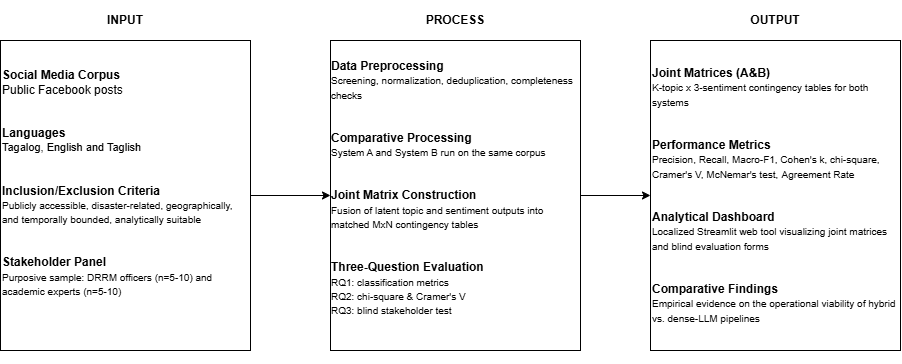
\includegraphics[width=0.9\textwidth]{figures/IPO.png}
	\caption{Input Process Output(IPO)}
	\label{fig:IPO}
\end{figure}

This study follows the common comparative pipeline that collects
disaster-related textual data, filters, preprocesses, and prepares it for
analysis by both systems. \sysA{} processes this corpus via Count
Vectorization, Latent Dirichlet Allocation (LDA), and \xlmr-based contextual
application, which are then combined into a joint matrix for further
evaluation. \sysB{} processes the same corpus using \qwen{} through structured
prompts for the same sentiment analysis and semantic assessment. The two
systems thus fall under a common data source, allowing for a comparative
evaluation to proceed.

The study’s textual disaster-related data is geographically linked to Bulacan and CAMANAVA, an area consisting of Caloocan, Malabon, Navotas, and Valenzuela during the study period of 2020-2025. The corpus includes social media content from government or disaster-management related public pages relative to the inclusion and exclusion criteria. The methodology identifies Bulacan and CAMANAVA as the geographic scope and specifies Tagalog, English, and Taglish as the principal language context of the textual data.


The study will apply a common measurement approach to the eligible corpus. Each
document is processed by both systems under their respective procedures. This
allows the resulting sentiments of both to be compared directly.

\subsection*{Research Question 1: Joint Matrix Latent Topic Structure and Sentiment Classification Relationship Analysis}

The first question of the study evaluates whether the latent topic structures
and sentiment classifications from the joint matrix of both \sysA{} and \sysB{}
demonstrate a measurable association with one another, and how this association
describes the dynamics between topics and sentiment classifications and
the strength of their relationships analytically. The study implements a
chi-square significance test to measure whether the relationship between the
topics and sentiment classifications exists, and a relationship strength
test with Fisher's Exact Test to measure the true strength of association between
topics and sentiment classifications and how big and impactful this is.

The independent relationship analysis of both systems is to be conducted with
the data inputs and $n$ specifications of potential latent topic topics to
create an equally sized joint matrix or contingency table. The analysis shall
report relevant relationship measurements of performance: the Chi-Square
Statistic and Fisher's Exact Test. The comparison emphasis is on determining
analytically the existence of a statistical relationship in their respective
joint matrices and the strength of their association independently produced by
both systems. Then they will be independently assessed against their
acceptability thresholds to conclude whether such a relationship exists and how
impactful it is on their evaluation of which words are being talked about
frequently together and how people feel about them, before comparing the two
systems again for further insights. Thresholds apply exclusively to independent
analysis.

\subsection*{Research Question 2: Sampled Comparative Evaluation}

The second question of the study examines both \sysA{} and \sysB{} through a
common evaluation corpus. The objective is to attain a representative output of
the two systems. It is to be structured to ensure representation of outcome
patterns where the two systems agree, where they disagree, and cases
representing different sentiment levels, where deemed appropriate.

The sampled documents from both systems are to be blindly evaluated by
stakeholders. This assessment will focus on their own assessment of the same
documents and their agreement or disagreement when presented in two blind tests
sampled from evaluated outputs that do not specify which is made by \sysA{} and
which is made by \sysB. It will be a assessment with human stakeholders. The two systems will
be evaluated individually in terms of stakeholder agreement rate and McNemar's
test. They will be evaluated independently and together when appropriate for
further insights. Acceptability thresholds are to be applied appropriately to
non-comparative measures.

\subsection*{Evaluation Framework}

The study utilises a same-measurement comparative evaluation framework in which
\sysA{} and \sysB{} are applied to the same corpus of disaster-related textual
data under comparable evaluation conditions. This framework is designed to
ensure that differences observed between the two systems are attributable to
their respective processing and analytical approaches rather than to the data
themselves.

The comparative process begins with the collection and preparation of an
eligible disaster-related textual corpus from Bulacan and CAMANAVA. The same
processed corpus is then provided to both systems according to their
respective procedures. \sysA{} applies LDA and an \xlmr-based joint matrix,
while \sysB{} processes the same textual input via \qwen{} using a predefined
prompting procedure. The resulting sentiment and latent topic outputs are recorded
via a common measurement structure established for the study.

The output of both systems is evaluated through three complementary analyses.
First, their sentiment classifications are assessed using performance measures
associated with Research Question 1. Second, their joint matrices are assessed
using performance measures associated with Research Question 2. Third, a
randomly selected sample of common outputs is subjected to blind stakeholder
evaluation in which their identities are concealed, and their outputs are
assessed under the same evaluation conditions.

\begin{figure}[htbp]
	\centering
	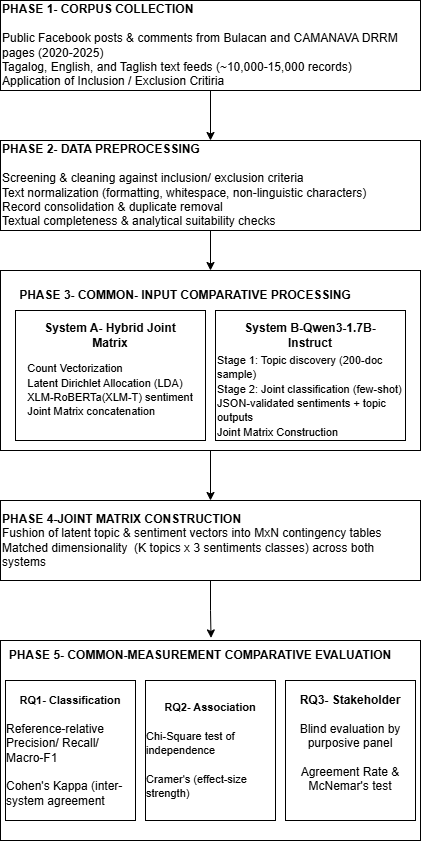
\includegraphics[width=0.7\textwidth]{figures/fig3_1_pipeline.png}
	\caption{Overall Research Pipeline}
	\label{fig:pipeline}
\end{figure}

This framework therefore is a common-input and comparative-analysis sequence.
Each system is evaluated either together or independently relative to
mathematical viability and consistency of measures of performance to gain
insights and findings. This allows the study to evaluate the independent ability
of each system and the relative performance of one over the other with respect
to the mathematical assumptions of each evaluation framework.

\section*{Data Sources and Corpus}

The textual data will be collected primarily from publicly accessible Facebook
posts and comments related to disasters occurring in Bulacan and CAMANAVA
during the study period of 2020-2025. Facebook is used as the principal data
source because posts and comments provide naturally occurring public
expressions that may contain information on public sentiment and perceived
disaster severity. The corpus will include textual content written in Tagalog,
English, and Taglish.

{\small
	\setlength{\tabcolsep}{3pt}
	\begin{longtable}{@{}
			l                                     % Agency / Location (natural width)
			l                                     % Region           (natural width)
			l                                     % User ID          (natural width)
			>{\raggedright\arraybackslash}p{5.75cm} % Facebook URL   (fixed, ragged-right)
			@{}}
		
		\caption{Target agencies and Facebook source pages used in the comparative flood analysis}
		\label{tab:target-agencies}\\
		
		\toprule
		\textbf{Agency / Location} & \textbf{Region} & \textbf{User ID} & \textbf{Facebook URL} \\
		\midrule
		\endhead
		
		\midrule
		\multicolumn{4}{r}{Continued on next page} \\
		\endfoot
		
		\bottomrule
		\endlastfoot
		
		% NOTE: rows transcribed from your screenshot; keep your own URL strings.
		Bulacan (General) & Bulacan & bulacan\_pdrrmo & \url{https://www.facebook.com/share/1EYVEuEk1i/?mibextid=wwXIfr} \\
		City of Malolos & Bulacan & malolos\_cdrrmo & \url{https://www.facebook.com/share/1D9yG4Ygq6/?mibextid=wwXIfr} \\
		City of Meycauayan & Bulacan & meycauayan\_cdrrmo & \url{https://www.facebook.com/share/1Gku63fZAq/?mibextid=wwXIfr} \\
		City of San Jose del Monte & Bulacan & csjdm\_cdrrmo & \url{https://www.facebook.com/share/1Di3r4DQXf/?mibextid=wwXIfr} \\
		City of Baliuag & Bulacan & baliuag\_cdrrmo & \url{https://www.facebook.com/share/1rUFil22ejY4/?mibextid=wwXIfr} \\
		Calumpit & Bulacan & calumpit\_mdrrmo & \url{https://www.facebook.com/share/1jNglrAcf7/?mibextid=wwXIfr} \\
		Hagonoy & Bulacan & hagonoy\_mdrrmo & \url{https://www.facebook.com/share/1hD7WknPQZ/?mibextid=wwXIfr} \\
		Marilao & Bulacan & marilao\_mdrrmo & \url{https://www.facebook.com/share/191rS6yyNg/?mibextid=wwXIfr} \\
		Bocaue & Bulacan & bocaue\_mdrrmo & \url{https://www.facebook.com/share/1BxkjNSc962/?mibextid=wwXIfr} \\
		Paombong & Bulacan & paombong\_mdrrmo & \url{https://www.facebook.com/share/1C4f8zAHnx/?mibextid=wwXIfr} \\
		Obando & Bulacan & obando\_mdrrmo & \url{https://www.facebook.com/share/1HmARF9TcY/?mibextid=wwXIfr} \\
		Bulakan & Bulacan & bulakan\_mdrrmo & \url{https://www.facebook.com/share/1QxQURuK69V/?mibextid=wwXIfr} \\
		Bustos & Bulacan & bustos\_mdrrmo & \url{https://www.facebook.com/share/1JNzjIK9TH4/?mibextid=wwXIfr} \\
		Plaridel & Bulacan & plaridel1\_mdrrmo & \url{https://www.facebook.com/share/1FImd5zyCY/?mibextid=wwXIfr} \\
		Pulilan & Bulacan & pulilan\_mdrrmo & \url{https://www.facebook.com/share/19TQHLEXRX/?mibextid=wwXIfr} \\
		Guiguinto & Bulacan & guiguinto\_mdrrmo & \url{https://www.facebook.com/share/1djYy9Ghab/?mibextid=wwXIfr} \\
		Pandi & Bulacan & pandi\_mdrrmo & \url{https://www.facebook.com/share/1GWb8GXpD7h/?mibextid=wwXIfr} \\
		Santa Maria & Bulacan & santamaria\_mdrrmo & \url{https://www.facebook.com/share/1CF9MHF83a/?mibextid=wwXIfr} \\
		San Miguel & Bulacan & sanmiguel\_mdrrmo & \url{https://www.facebook.com/share/19fRTlWvuA/?mibextid=wwXIfr} \\
		San Ildefonso & Bulacan & sanildefonso\_mdrrmo & \url{https://www.facebook.com/share/1c83yUQ9R/?mibextid=wwXIfr} \\
		San Rafael & Bulacan & sanrafael\_mdrrmo & \url{https://www.facebook.com/share/19VnxKnack/?mibextid=wwXIfr} \\
		Angat & Bulacan & angat\_mdrrmo & \url{https://www.facebook.com/share/1JbkbF9PpT/?mibextid=wwXIfr} \\
		Norzagaray & Bulacan & norzagaray\_mdrrmo & \url{https://www.facebook.com/share/1DVq0VAd1B/?mibextid=wwXIfr} \\
		Doña Remedios Trinidad & Bulacan & drt\_mdrrmo & \url{https://www.facebook.com/share/1G2Yq16Fec/?mibextid=wwXIfr} \\
		Valenzuela City & CAMANAVA & valenzuela\_cdrrmo & \url{https://www.facebook.com/share/1Gku63fZAq/?mibextid=wwXIfr} \\
		Malabon City & CAMANAVA & malabon\_cdrrmo & \url{https://www.facebook.com/share/1ELBPLYcVsJ/?mibextid=wwXIfr} \\
		Navotas City & CAMANAVA & navotas\_cdrrmo & \url{https://www.facebook.com/share/1D6gb4XR6w/?mibextid=wwXIfr} \\
		Caloocan City & CAMANAVA & caloocan\_cdrrmo & \url{https://www.facebook.com/share/1F78Zh77BW/?mibextid=wwXIfr} \\
		
	\end{longtable}
} % end
\small

Data collection will be a semi-automated manual extraction procedure supported
by a web scraper browser extension to aid in extracting the textual data from
posts and their comment threads. The relevant Facebook posts and their
available comments will be identified using the study's own inclusion and
exclusion criteria. The web scraper extension will assist in the extraction and
organization of available data, while manual procedures will identify relevant
sources.

\begin{longtable}{@{}p{0.22\textwidth} p{0.22\textwidth} p{0.22\textwidth} p{0.30\textwidth}@{}}
	\caption{Keywords used for disaster and flood detection in the social media scraper}\label{tab:keywords}\\
	\toprule
	\textbf{Category} & \textbf{English Keyword} & \textbf{Tagalog/Local Term} & \textbf{Description} \\
	\midrule
	\endfirsthead
	
	\caption[]{Keywords used for disaster and flood detection in the social media scraper (continued)}\\
	\toprule
	\textbf{Category} & \textbf{English Keyword} & \textbf{Tagalog/Local Term} & \textbf{Description} \\
	\midrule
	\endhead
	
	\midrule
	\multicolumn{4}{r}{Continued on next page} \\
	\endfoot
	
	\bottomrule
	\endlastfoot
	
	Historical Events & Typhoon Ulysses & Bagyo & Major tropical cyclone event \\
	Historical Events & Typhoon Rolly & Bagyo & Major tropical cyclone event \\
	Historical Events & Typhoon Quinta & Bagyo & Major tropical cyclone event \\
	Historical Events & Typhoon Fabian & Bagyo & Major tropical cyclone event \\
	Historical Events & Typhoon Karding & Bagyo & Major tropical cyclone event \\
	Historical Events & Typhoon Paeng & Bagyo & Major tropical cyclone event \\
	Historical Events & Typhoon Egay & Bagyo & Major tropical cyclone event \\
	Historical Events & Typhoon Carina & Bagyo & Major tropical cyclone event \\
	Water & Flooding & Pagbaha & Flooding condition \\
	Water & Flood & Baha & Flood event \\
	Water & Flash flood & Biglaang baha & Sudden flood surge \\
	Water & Submerged & Lubog sa baha / Lubog & Waterlogged or submerged area \\
	Water & Overflow & Umaapaw / Umapaw & Water exceeds capacity \\
	Water & High Tide & Taib & Coastal water surge \\
	Water & Dam release & Pagpapakawala ng tubig & Controlled drainage from dam \\
	Water & Spillway & Spillway & Floodwater release outlet \\
	Weather & Rainfall & Buhos ng ulan & Heavy rainfall \\
	Weather & Rain & Ulan & Rainfall \\
	Weather & Heavy Rain & Malakas na ulan & Intense rainfall \\
	Weather & Thunderstorm & Kidlat at kulog & Storm with lightning \\
	Weather & Monsoon & Habagat / Amihan & Seasonal wind and rain pattern \\
	Weather & Low Pressure Area & LPA & Weather disturbance \\
	Rescue & Rescue & Saklolo / Sagip & Emergency rescue action \\
	Rescue & Help & Tulong & Assistance request \\
	Rescue & Evacuate & Lumikas & Leaving threatened area \\
	Rescue & Evacuation & Paglikas / Likas & Mass movement to shelter \\
	Rescue & Evacuation Center & Sentro ng paglikas & Shelter for evacuees \\
	Rescue & Trapped & Na-trap / Nakulong & Unable to evacuate \\
	Rescue & Stranded & Naipit & Stuck due to flood or weather \\
	Rescue & Missing & Nawawala & Missing persons report \\
	Rescue & Casualty & Nasawi / Patay & Fatality or death \\
	Rescue & Relief goods & Ayuda & Aid and support delivered \\
	Warning & Advisory & Abiso & Public warning \\
	Warning & Alert & Alerto & Warning alert issued \\
	Warning & Hazard & Panganib & Hazard threat \\
	Warning & Red Warning Level & Red Warning Level & Severe alert status \\
	Warning & Orange Warning Level & Orange Warning Level & Moderate-to-high alert status \\
	Warning & Yellow Warning Level & Yellow Warning Level & Precautionary alert status \\
	Warning & Signal No. 1 & Signal No. 1 & Weather warning signal \\
	Warning & Signal No. 2 & Signal No. 2 & Weather warning signal \\
	Warning & Signal No. 3 & Signal No. 3 & Weather warning signal \\
	Warning & Signal No. 4 & Signal No. 4 & Weather warning signal \\
	Warning & Signal No. 5 & Signal No. 5 & Weather warning signal \\
	Threat & Landslide & Pagguho ng lupa & Slope failure event \\
	Threat & Class suspension & Walang pasok / Suspindido ang klase & School closure due to hazard \\
	Threat & Threatening & Nagbabanta & Risk or threat warning \\
	Infrastructure & Angat Dam & Angat Dam & Dam infrastructure \\
	Infrastructure & Bustos Dam & Bustos Dam & Dam infrastructure \\
	Infrastructure & Ipo Dam & Ipo Dam & Dam infrastructure \\
\end{longtable}

The data sourcing will target an approximate corpus size of 10,000-15,000
records and above. It will source from publicly available pages of
disaster-related agencies around Bulacan and CAMANAVA, with optional inclusions
of newer agencies and wider public government pages. The timeframe of
2020-2025 was chosen to obtain relevant qualitative data that is relatively
not out of date and is feasible to attain.

\subsection*{Inclusion Criteria}

Facebook posts or comments are to be included if they satisfy the following
criteria: they are publicly accessible; they are related to a disaster,
disaster event, disaster impact, response, recovery, or other related topics;
they are relevant to Bulacan or CAMANAVA; they fall within the 2020--2025
study period; they contain textual content suitable for sentiment and semantic
analysis; and they are written in Tagalog, English, or Taglish.

\subsection*{Exclusion Criteria}

Facebook posts or comments are to be excluded when they are not publicly
accessible; when they are not related to a disaster, disaster event, disaster
impact, response, recovery, or other related topics; when they fall outside the
scope of Bulacan or CAMANAVA; when they fall outside the 2020--2025 study
period; when they contain no textual content suitable for sentiment and
semantic analysis; when they consist entirely of spam, advertisements,
promotional materials, and other unrelated content; when they are duplicated
records bearing the same content or corrupted text; and when they contain any
mentions, hashtags, private information, or emojis.

\begin{table}[htbp]
	\centering
	\caption{Inclusion and Exclusion Criteria for Facebook Posts and Comments}
	\label{tab:screening_criteria}
	\begin{tabular}{p{0.5cm} p{3.2cm} p{5.2cm} p{5.2cm}}
		\toprule
		\textbf{\#} & \textbf{Dimension} & \textbf{Inclusion Criteria} & \textbf{Exclusion Criteria} \\
		\midrule
		1 & Accessibility      & Publicly accessible & Not publicly accessible \\
		2 & Topical relevance  & Related to disaster, disaster impact, response, recovery, or related topics & Unrelated to disasters or related topics \\
		3 & Geographic scope   & Relevant to Bulacan or CAMANAVA & Outside the scope of Bulacan or CAMANAVA \\
		4 & Time frame         & Within the 2020--2025 study period & Outside the 2020--2025 study period \\
		5 & Text suitability   & Text suitable for sentiment and semantic analysis & No suitable textual content \\
		6 & Language           & Tagalog, English, or Taglish & Other languages \\
		7 & Content quality    & --- & Entirely spam, advertisements, or promotional content \\
		8 & Record integrity   & --- & Duplicated or corrupted records \\
		9 & Privacy/formatting & --- & Contains mentions, hashtags, private information, or emojis \\
		\bottomrule
	\end{tabular}
\end{table}

Together, the resulting eligible records constitute the common corpus used by
both \sysA{} and \sysB{} under their individual procedures, so that differences
in sentiment and topic outputs can be examined under a common data basis.

\section*{Data Preprocessing}

The collected common corpus is to undergo preprocessing before being submitted
to \sysA{} and \sysB, with the intention of removing irrelevant content while
preserving linguistic information necessary for sentiment and latent topic
analysis. The prepared corpus is to be sent to both systems to remain
consistent with the comparative analysis framework. The records are to be
screened and cleaned based on the inclusion criteria; any content that falls
within the exclusion criteria is to be excluded and removed. Text normalization
is to be done next to improve consistency; this will remove formatting
artifacts, excessive whitespace, and other characters that are not relevant to
the study. Record consolidation is to be done afterward to remove remaining
duplicates. Finally, the corpus is to be subjected to textual completeness and
analytical suitability checks before being fed to the two systems.

\section*{Comparative Systems}

This study evaluates two computational systems for disaster-related sentiment
and latent topic analysis: \sysA, a hybrid LDA--\xlmr{} Joint Matrix System, and
\sysB, Qwen3-1.7B-Instruct-Q4\_K\_M. Though the two different systems employ different processing
approaches, both receive the same prepared disaster-related textual corpus and
produce sentiment and latent topic outputs that are evaluated using the common
measurement framework of the study. This arrangement allows the study to
distinguish differences arising from the analytical approaches of the systems
while maintaining a common basis for comparison.

\subsection*{System A: LDA-XLM-RoBERTa Joint Matrix System}

\sysA{} employs a hybrid approach that combines Count Vectorization, Latent
Dirichlet Allocation (LDA), and \xlmr-based contextual representations into a
joint matrix. Count Vectorization provides the lexical representation of the
textual corpus, while LDA is used to derive topic-related representations from
the processed documents. \xlmr{} provides contextual language representation
for sentiment analysis of the disaster-related text. These representations are
integrated into a joint matrix that serves as the computational representation
for the subsequent analysis.

\subsubsection{Count Vectorization}

Count Vectorization is the process of converting text documents into numerical
vectors that allow machine learning models to perform natural language
processing (NLP). This starts with removing unnecessary elements such as
punctuation, URLs, and numbers; all text is also converted to lowercase. The
model processes them by splitting the documents into words so that the model
can understand and analyze each word individually, followed by identifying
unique words from the preprocessed text. This serves as the reference that maps
text into a numerical vector. The text is then converted into numerical vectors
for the machine learning model to process. It acts as a bridge between human
language and machine language \parencite{kozhevnikov2020}. Vectorization is a function that maps a text document into a numerical vector
in a high-dimensional space. 

\subsubsection{Latent Dirichlet Allocation (LDA)}

Latent Dirichlet Allocation is a generative probabilistic model of a corpus. The
assumption is that each document is represented as a random mixture over
topics, and each of these topics is characterized by a distribution of
words. Its generative process follows that, for each document $d$ in the
corpus:

\begin{enumerate}[label=\arabic*.]
	\item Choose $\theta_d \sim \operatorname{Dirichlet}(\alpha)$.
	\item Choose $\phi_k \sim \operatorname{Dirichlet}(\beta)$ for each topic
	$k \in \{1,\dots,K\}$.
	\item For each of the $N_d$ words $w_{d,n}$:
	\begin{enumerate}[label=\alph*.]
		\item Choose a topic $z_{d,n} \sim \operatorname{Multinomial}(\theta_d)$.
		\item Choose a word $w_{d,n} \sim p(w_{d,n} \mid z_{d,n}, \beta)$, a
		multinomial probability conditioned on the topic.
	\end{enumerate}
\end{enumerate}

Each document draws its overall topic mixture $\theta_d$ from a Dirichlet
distribution parameterized by $\alpha$ Given the parameters $\alpha$ and $\beta$. The parameters of the LDA get modified depending on their level. Overall, the
model has three levels: corpus level, document level, and word level. The
parameters $\alpha$ and $\beta$ are corpus-level parameters and are sampled once
in the process of generating a corpus. The variables $\theta_d$ are
document-level variables and are sampled once per document. Finally, the
variables $z_{d,n}$ and $w_{d,n}$ are word-level variables and are sampled once
per word in each document \parencite{blei2003}.

\subsubsection{Latent Dirichlet Allocation (LDA) $K$-Topic Selection}

The number of $K$ topics was selected empirically through a coherence
sweep across $K \in \{2,3,\dots,K_{\max}\}$. For each value of $K$, the model
was fitted on the prepared corpus with a fixed random state of 42, batch
learning, and 100 maximum iterations, and the mean UMass Coherence score and
its respective criterion determined the $K$-topic quantity of the model.

The UMass coherence score evaluates the quality of the topic models. It relies
on the internal corpus of the model, and words are calculated in order of their
frequency within the topic; the expected outcome is negative, with values
nearest to zero being better. To compute the UMass coherence score:
\begin{equation}
	C_{\mathrm{UMass}}(T_k)
	= \sum_{m=2}^{N} \sum_{n=1}^{m-1}
	\log \frac{D(w_m, w_n) + 1}{D(w_n)}
	\label{eq:umass}
\end{equation}
where $T_k = \{w_1, w_2, \dots, w_N\}$ is the list of $N$ probable words in
topic $k$, $D(w_m, w_n)$ is the number of documents in the corpus containing
both $w_m$ and $w_n$, and $D(w_n)$ is the number of documents containing $w_n$.
This metric relies on co-occurrence statistics gathered from the corpus being
modeled and is domain specific \parencite{mimno2011}.

Because the sentiment category has exactly three categories. The selected $K$---the UMass coherence score nearest to
zero among the sampled values---will be the selected amount of $K$-topics for
the LDA configuration and the amount of topics for \sysB's Stage 1, to preserve
the matched dimensionality of their joint matrices required for the comparative
evaluation framework.

\subsubsection{XLM-RoBERTa (XLM-T)}

LDA only gives us a platform to conduct latent semantic analysis; it only
allows us to see which words co-occur relative to a given corpus. It does not
tell us whether people talk about these sets of words or topics negatively,
positively, or neutrally. Sentiment analysis utilizing language models in
multilingual settings makes this possible. XLM-T is a transformer-based model
that is an extension of \xlmr{} trained on social media posts on X (formerly
Twitter). The model is trained on 198 million social media posts that include
English, Tagalog, and many more, with Tagalog/Filipino comprising roughly one
million posts \parencite{barbieri2021}.

Following pretraining, XLM-T was fine-tuned for sentiment classification on
human-annotated datasets in eight core languages: Arabic, English, French,
German, Hindi, Italian, Portuguese, and Spanish. Tagalog/Filipino is not among
these eight fine-tuning languages. Instead, Tagalog sentiment classification is
supported via zero-shot cross-lingual transfer. Because the pretraining stage
learns a shared multilingual representation, sentiment supervision from the
eight core languages generalizes to Tagalog without any Tagalog sentiment labels
being used during training. This modification allows XLM-T to outperform other
multilingual NLP transformer-based models that rely on more formal training data
such as Wikipedia and CommonCrawl \parencite{barbieri2021}.

\begin{figure}[htbp]
	\centering
	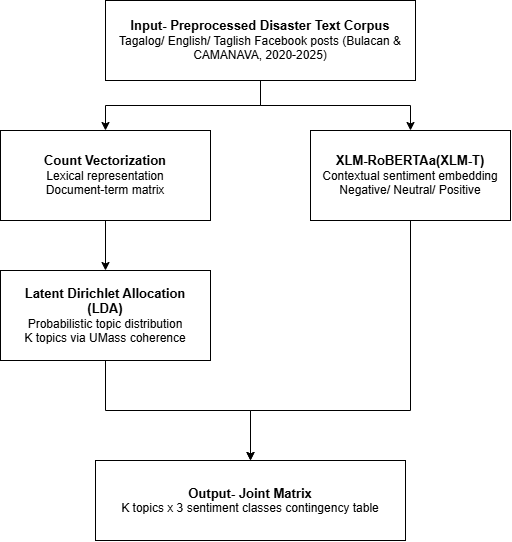
\includegraphics[width=0.9\textwidth]{figures/fig3_2_systemA.png}
	\caption{System A Architecture}
	\label{fig:systemA}
\end{figure}

The system generates sentiment classifications using the defined ternary
sentiment categories of Negative, Neutral, and Positive, as well as the
topics and their respective words. These outputs are fixed before the
comparative evaluation.

\subsection*{System B: \texttt{Qwen3-1.7B-Instruct-Q4\_K\_M}}

\sysB{} employs \qwen{} as a few-shot language model for disaster-related
sentiment and latent topic analysis. Unlike \sysA, which is a hybrid approach
utilising multiple representations, \sysB{} processes the textual inputs
directly through a predefined prompting procedure.

Large language models are transformer-based neural networks
\parencite{vaswani2017} trained on very large text collections. Their attention
mechanism computes each token's representation from the other tokens, so the
model uses context from the whole post, which helps with informal and
code-switched text. They also show in-context learning: given a task
description and a few labeled examples in the prompt, they can do a new task
without any parameter updates \parencite{brown2020}.

System B uses \qwen, a 4-bit quantized, open-weight (Apache 2.0) model
\parencite{yang2025}. Qwen3 expanded language coverage from 29 to 119 languages
and dialects, which is relevant to Tagalog and English but does not by itself
show strong Taglish performance. Quantization saves memory at a possible cost
in accuracy.


The prompting procedure specifies the required sentiment categories and topics
output format to ensure consistency and that comparative analysis assumptions
are respected. For sentiment analysis, the system produces one of the three
defined categories: Negative, Neutral, or Positive.

\subsubsection{Model Specifications}

\sysB{} utilizes the Qwen3-1.7B-Instruct model in GGUF format at Q4\_K\_M
quantization. Inference is performed with temperature at 0.1 and a top-$p$ of
1.0. It has a maximum generation length of 48 tokens. This low temperature
reduces sampling variance across documents and supports reproducibility of the
classification outputs.

\subsubsection{Two-Stage Prompting Architecture}

\sysB{} operates in two stages: topic discovery and joint classification. This
separation is crucial, as the model must first establish the canonical topic
taxonomy before it can assign topic labels to individual documents. The number
is fixed to the value of the $K$-topic to match \sysA's LDA dimensionality,
which guarantees that the joint matrix (topic--sentiment contingency table) of
both systems has the same matrix shape and is legible for the common
measurement framework.

\paragraph{Stage 1: Topic Discovery.}
In the first stage, a representative sample of 200 documents is drawn from the
prepared corpus. This representative sample is presented to the model with
instructions to synthesize a canonical taxonomy of distinct $K$ topics. The
prompt directs the model to focus on core actions, problems, or topics rather
than proper nouns, locations, or geographic identifiers. Each topic must have a
short label and a set of keywords extracted from the representative sample.

\begin{figure}[htbp]
	\centering
	\label{ls:stage-1-prompt}
	\begin{minipage}{0.9\textwidth}
		\begin{lstlisting}[language=Python,
			showspaces=false,
			showstringspaces=false,
			caption={Stage 1 Prompt}]
TOPIC_DISCOVERY_SYSTEM ="""
You are an expert qualitative data analyst. Your task is to analyze a batch of text documents and synthesize a canonical taxonomy of exactly {n_topics} distinct topics.
			
GUIDELINES:
- Focus on the core ACTION, PROBLEM, or THEME (e.g., medical relief, structural damage, supply distribution).
- Strictly omit all proper nouns, locations, regions, and geographic identifiers.
- Each topic must have a short 'label' (2-4 lowercase words), and actual 'keywords' (bag-of-words) extracted directly from the texts.
- Respond ONLY with a valid JSON array of objects. No markdown, no explanations.
- CRITICAL: Your output MUST start with "[" and end with "]".
			
EXAMPLE OUTPUT:
[
{{"label": "rescue efforts", "keywords": ["rescue", "stranded", "volunteer", "bagal", "rescuers"]}},
{{"label": "flood impact", "keywords": ["baha", "tubig", "lubog", "taas", "stranded"]}},
{{"label": "health risks", "keywords": ["leptospirosis", "sintomas", "check-up", "baho"]}}
]
/no_think
"""
			
TOPIC_DISCOVERY_USER = """
Here is a representative sample of {n_docs} documents from the dataset:
			
{documents_block}
			
Generate the JSON array of exactly {n_topics} topics based on the themes present in these documents.
JSON Output:
"""
		\end{lstlisting}
	\end{minipage}
\end{figure}

The model returns a JSON array of topic objects. The prompt enforces strict
JSON output with no markdown or explanations. This discovered taxonomy is
validated for structural completeness before being used in Stage 2. The final
taxonomy is recorded to a CSV file and is used for the common measurement
framework.

The discovery sample is drawn using random sampling from the whole prepared
corpus. This rule is fixed to prevent bias toward the first entries in the
corpus being sampled first.

\paragraph{Stage 2: Joint Sentiment and Topic Classification.}
In the second stage, each document in the prepared corpus is classified
individually. The prompt presents the model with the final taxonomy from
Stage 1 and a small set of few-shot examples demonstrating the sentiment
decision rule. The model is required to output a single JSON object with two
fields: \texttt{sentiment} and \texttt{topic}.

The sentiment must be exactly one of the following: \texttt{POS(Positive)},
\texttt{NEG(Negative)}, or \texttt{NEU(Neutral)}. The prompt defines the following as:
\begin{itemize}
	\item \texttt{POS}: the text expresses joy, gratitude, hope, relief, or praise;
	\item \texttt{NEG}: the text expresses anger, sadness, fear, frustration, or criticism;
	\item \texttt{NEU}: the text is purely informational, factual, asking for
	help, or expresses a balanced or mixed view.
\end{itemize}

\begin{figure}[htbp]
	\centering
	\label{ls:stage-2-prompt}
	\begin{minipage}{0.9\textwidth}
		\begin{lstlisting}[
			language=Python,
			showspaces=false,
			showstringspaces=false,
			caption={Stage 2 Prompt}]
JOINT_SYSTEM = """
You are an expert analyst classifying social media posts. You must output TWO labels: SENTIMENT and TOPIC.
			
SENTIMENT must be exactly one of: "POS", "NEG", "NEU".
- POS: The text expresses joy, gratitude, hope, relief, or praise.
- NEG: The text expresses anger, sadness, fear, frustration, or criticism.
- NEU: The text is purely informational, factual, or expresses a balanced/mixed view. Do not assume factual requests are negative.
			
TOPIC must be exactly one of the 'label' values from the provided taxonomy list.
			
Respond ONLY with a valid JSON object. No markdown, no explanations.
FORMAT:
{{"sentiment": "LABEL", "topic": "exact topic label from list"}}
/no_think
"""
			
JOINT_USER = """Available taxonomy (label and description): {topic_list_with_descriptions}
			
Examples:
Text: "Salamat sa mga rescuers! Ligtas na kami."
JSON: {{"sentiment": "POS", "topic": "rescue efforts"}}
			
Text: "Base sa PAGASA, tuloy-tuloy ang ulan hanggang weekend. Maghanda po."
JSON: {{"sentiment": "NEU", "topic": "flood warning"}}
			
Text: "Nakakagalit! Ang bagal ng rescue. Ilang oras na kaming stranded."
JSON: {{"sentiment": "NEG", "topic": "flood impact"}}
			
Text to classify:"{text}"
			
JSON Response:
"""
		\end{lstlisting}
	\end{minipage}
\end{figure}

The prompt explicitly instructs the model not to assume that factual requests
are negative, addressing a common failure mode in disaster text classification.
The \texttt{topic} field must be exactly one of the label values from the
discovered taxonomy. As in Stage 1, the model is instructed to output only
valid JSON with no markdown or explanations.

\begin{figure}[htbp]
	\centering
	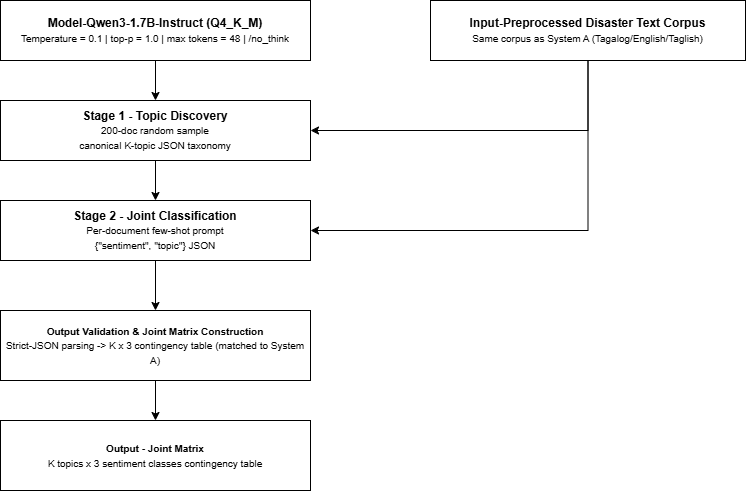
\includegraphics[width=0.9\textwidth]{figures/fig3_3_systemB.png}
	\caption{System B Architecture}
	\label{fig:systemB}
\end{figure}

Both systems are therefore applied to the same processed corpus but retain their
individual internal procedures. Their outputs are to be subjected to the same
evaluation framework for independent assessment and comparative analysis.

\section*{End Products of System A and System B: The Joint Matrix}

In order for both systems to undergo the same measurement comparative analysis,
both their latent topic matrices and their sentiment classification matrices
must be fused together onto a single joint matrix that has the same dimension
and size. This will allow quantifiable measurements of performance to be
performed on both systems' outputs independently and relative to one another.

Contingency tables allow the evaluation of the joint distributions, frequency
counts, and percentages of two categorical variables. Formally, the table
variables define the rows and columns, one variable defining the rows of the
table and another variable defining the columns of the table \parencite{ncssnd}.

Let $T = \{\topic{1}, \dots, \topic{M}\}$ be the row variable of topics
with $M$ topics, and $S = \{\sent{1}, \dots, \sent{N}\}$ be the column variable
of sentiment classifications with $N$ classes. Then an $M \times N$ contingency
table with marginal totals is defined as
\begin{equation}
	J =
	\begin{pmatrix}
		j_{11}   & j_{12}   & \cdots & j_{1n}   & n_{1n} \\
		j_{21}   & j_{22}   & \cdots & j_{2n}   & n_{2n} \\
		\vdots   & \vdots   & \ddots & \vdots   & \vdots \\
		j_{m1}   & j_{m2}   & \cdots & j_{mn}   & n_{mn} \\
		n_{m1}      & n_{m2}      & \cdots & n_{mn}      & n
	\end{pmatrix}
	\label{eq:jointmatrix}
\end{equation}
where each cell entry is defined as
\begin{equation}
	j_{mn} = \bigl|\{\, d \in \mathcal{D} : t(d) = \topic{m} \;\wedge\; s(d) = \sent{n} \,\}\bigr|
	\label{eq:cellentry}
\end{equation}
with $t(d)$ representing the assigned latent topic of document $d$ and $s(d)$
representing its assigned sentiment classification.

\section*{Measurement and Evaluation}

The information collected from the two systems will be processed, coded, and
analysed with suitable performance measures that correspond to the three
research questions of this investigation. System A, the Hybrid LDA + XLM-RoBERTa Joint
Matrix System, and System B, $Qwen3-1.7B-Instruct-Q4\_K\_M$, will be assessed using the exact evaluation
framework to ensure comparative integrity in the evaluation results. Each
statistic will be run separately on each system prior to comparing and making
relative findings.

\subsection*{System Implementation: The Analytical Dashboard}

To operationalize the backend computational pipelines of System A and System B for both analytical visualization
and stakeholder evaluation, a localized web dashboard is developed. While the core processing relies on heavy backend machine learning operations (LDA, XLM-RoBERTa, and Qwen3 interface), the dashboard provides a graphical user interface (GUI) that translates these mathematical output into interactive visual analytics.

Guided by sensemaking theory, the backend computational pipelines are encapsulated within a localized analytical web dashboard. While System A and System B perform the heavy mathematical workload of vectorization and probabalistic modeling. The dashboard provides the necessary visual interface for human-in-the-loop validation. It translates abstract joint matrices and evaluated corpus into interactive charts and blinded evaluation forms, enabling local stakeholders to visually verify the alignment between disaster topics and community sentiments.

The dashboard will have these primary modules:
\begin{enumerate}
	\item \textbf{Corpus and Pipeline Ingestion Module.} This module handles 
	the loading of the pre-processed, cleaned corpus and executes the backend 
	pipelines of System A and System B. It manages the generation of the 
	Joint Matrices and stores the resulting sentiment and topic classifications 
	in structured data formats (CSV) for frontend rendering.
	
	\item \textbf{Visual Analytics and Joint Matrix Module.} This module 
	renders the mathematical outputs of the study. It displays interactive 
	bar charts for sentiment distributions, topic-word probability heatmaps, 
	and the $M \times N$ Joint Matrix contingency tables. This allows the 
	researchers and technical experts (Cohort B) to visually validate the 
	coherence of the LDA topics and the alignment of the sentiment 
	classifications without parsing raw code.
	
	\item \textbf{Blind Evaluation Instrument Module.} To execute Research 
	Question 2, the dashboard features a specialized evaluation interface. 
	It randomly samples documents from the corpus and presents the 
	system-generated sentiment and topic classifications side-by-side in a 
	blinded format (labeled only as ``Output X'' and ``Output Y''). The 
	stakeholder panel (Cohort A and B) interacts directly with this web 
	interface, utilizing a assessment format GUI to record their agreement or 
	disagreement. The dashboard automatically logs these interactions into 
	a secure database for the subsequent McNemar's Test and other computations.
\end{enumerate}

By utilizing a lightweight python web framework, the dashboard ensures the the system remains entirely dependent on local backend environment satisfying the need for
an interactive visual analytical system.

\subsection*{Decision Support System (DSS)}

Decision Support System (DSS) was first introduced as a system designed to aid decision makers in semi-structured issues that algorithms cannot resolve. It served to increase the managers capabilities rather than replace them in the decision making process. DSS provides a quantitative basis that supports managerial decisions instead of solely relying on personal intuition and experience~\cite{Rashidi2018}.

A standard Decision Support System framework consists of four primary components:
\begin{enumerate}
	\item \textbf{Language System (LS):} Interprets recognizable messages.
	\item \textbf{Presentation System (PS):} Manages all messages made by decision support systems.
	\item \textbf{Knowledge System (KS):} Acts as the repository of integrated information within DSS.
	\item \textbf{Problem-Processing System (PPS):} Acts to resolve the problem.
\end{enumerate}

To integrate topics and sentiment analysis into a DSS, unstructured text is collected from sources such as Twitter, Amazon, and Google Reviews. Preprocessing is applied to remove URLs, hashtags, usernames, special characters, stop words, and fake news. Topic modeling techniques, such as Latent Dirichlet Allocation (LDA), are then utilized to identify the discussed topics.

Furthermore, sentiment analysis—using lexicon-based tools (e.g., VADER, SentiWordNet, TextBlob), machine learning models (e.g., SVM, Naive Bayes, LSTM), or hybrid approaches—is implemented to determine the sentiment associated with each topic. Two common integration methods include:
\begin{itemize}
	\item Executing LDA prior to sentiment analysis to assign each document to its dominant topic and calculating the average sentiment for every topic.
	\item Implementing Aspect-Based Sentiment Analysis (ABSA).
\end{itemize}

The resulting output is a matrix mapping topics against sentiment scores along with volume and trend metrics. In the decision layer, this output is utilized in Multi-Criteria Decision Making (MCDM) to rank services in Importance-Performance Analysis (IPA) to determine priorities, predict demand, and assess business reputation~\parencite{AguilarMoreno2024}. Lastly, the insights appear on a dashboard featuring real-time monitoring and alerts.

When implementing this framework, sentiment analysis limitations must be considered, including sarcasm and irony, domain-specific jargon, multiple sentiments within a single sentence, and the English-centric design of most existing tools, which necessitates custom training data for languages such as Filipino or Taglish. Additionally, consulting the original articles is recommended for specific implementation details~\parencite{AguilarMoreno2024}.

The system will utilize decision support system to help local stakeholders find topics that has to be investigated due to frequency distribution of their sentiment classifications (high levels of negative and positive sentiment but minimal neutral sentiments, high concentration of sentiment classifications sentiments towards a single class and such). It also helps local stakeholders make informed decisions on which topics should they focus their time, consultations, expertise and other resources to have an aligned response with what people talk about in social networks and how they feel talking about it.

\subsection*{Waterfall Development Methodology}

The Waterfall model is a plan-driven software process in which development
moves through requirements, design, implementation, verification, and
maintenance in sequence \parencite{sommerville2016}. The model suits projects whose requirements are well
understood and unlikely to change, and it produces clear documentation at the
end of each phase \parencite{pressman2020}.

SAKLOLO fits these conditions. The disaster types, sentiment categories, the
two systems, the evaluation metrics, and the inclusion and exclusion criteria
are defined in this proposal before implementation begins. Because the study
compares two fixed systems on a fixed corpus, changes in the middle of
development would also weaken the comparison.

The phases map onto the study as follows.

\paragraph{Requirements analysis.} The corpus criteria (public Facebook posts
and comments in Tagalog, English, and Taglish about natural disasters in
Bulacan and CAMANAVA, 2020 to 2025), the common output format, and the
evaluation metrics are fixed. The deliverable is the finalized scope and
evaluation plan.

\paragraph{System design.} The System A and System B architectures, the Joint
Matrix, and the dashboard layout are specified. The deliverable is the
architecture diagrams and the data schema.

\paragraph{Implementation.} The data pipeline (collection, cleaning,
anonymization), the two systems, the evaluation scripts, and the dashboard are
built. The deliverable is the working prototype.

\paragraph{Testing and verification.} Outputs are checked against the common
format, both systems are run on the same corpus, the statistical analyses are
computed, and the blind stakeholder evaluation is conducted. The deliverable is
the results tables and test report.

\paragraph{Maintenance.} Documentation is completed and recommendations for
future work are recorded. Because the study excludes real-time integration into
DRRM command centers, maintenance is limited to documentation and handover.

\begin{figure}[htbp]
	\centering
	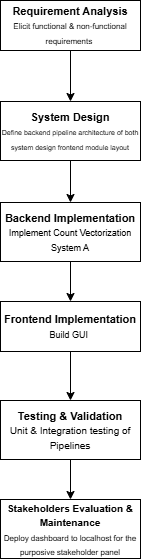
\includegraphics[width=0.3\textwidth]{figures/waterfall.png}
	\caption{Waterfall Development Model}
	\label{fig:waterfall}
\end{figure}

A known weakness of Waterfall is its limited flexibility once a phase is
complete \parencite{sommerville2016}, which is reduced here by fixing the
requirements and metrics in advance.

\subsection*{System Flowchart}
\begin{figure}[htbp]
	\centering
	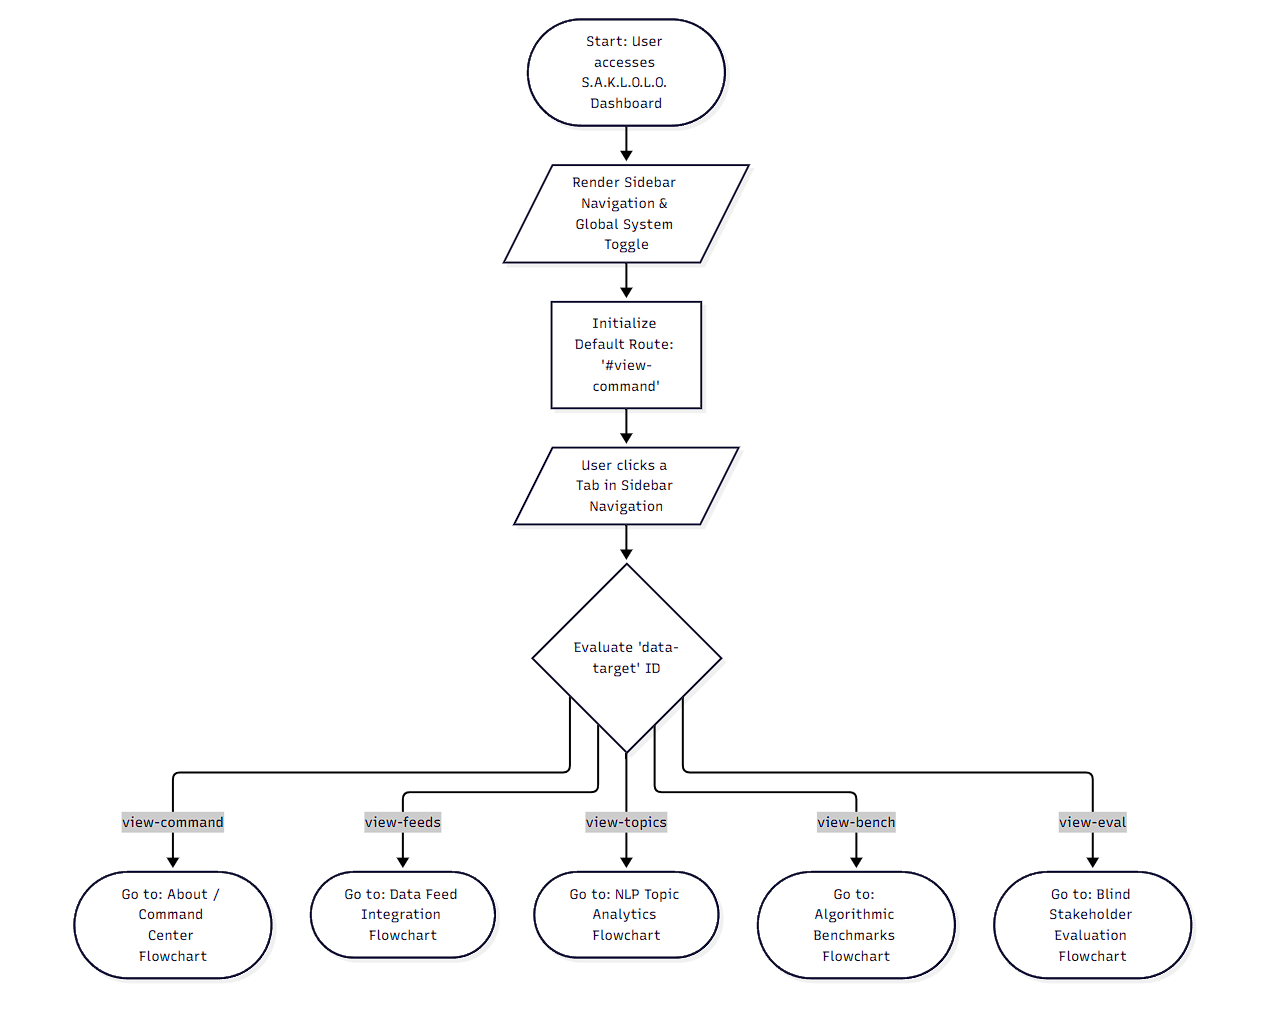
\includegraphics[width=0.9\textwidth]{figures/image2.png}
	\caption{Master dashboard navigation}
	\label{fig:Master_navigation}
\end{figure}

The system is a single page application,
that utilizes the sidebar to trigger state changes that will direct the user to their respective sub-modules.

\begin{figure}[htbp]
	\centering
	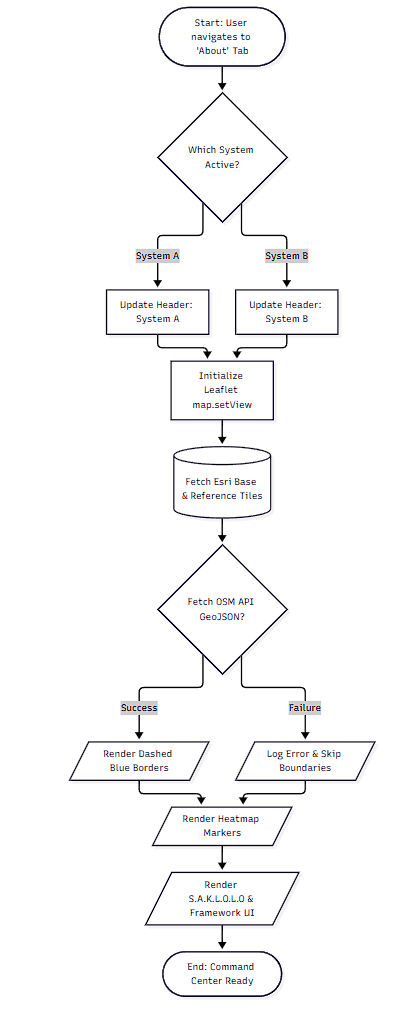
\includegraphics[width=0.5\textwidth]{figures/image5.png}
	\caption{View Command}
	\label{fig:view command}
\end{figure}

This figure \ref{fig:view command}  outlines the initialization sequence for the Leaflet maps, dynamic OSM boundary fetching, and the rendering of the SAKLOLO evaluation framework.

\begin{figure}[htbp]
	\centering
	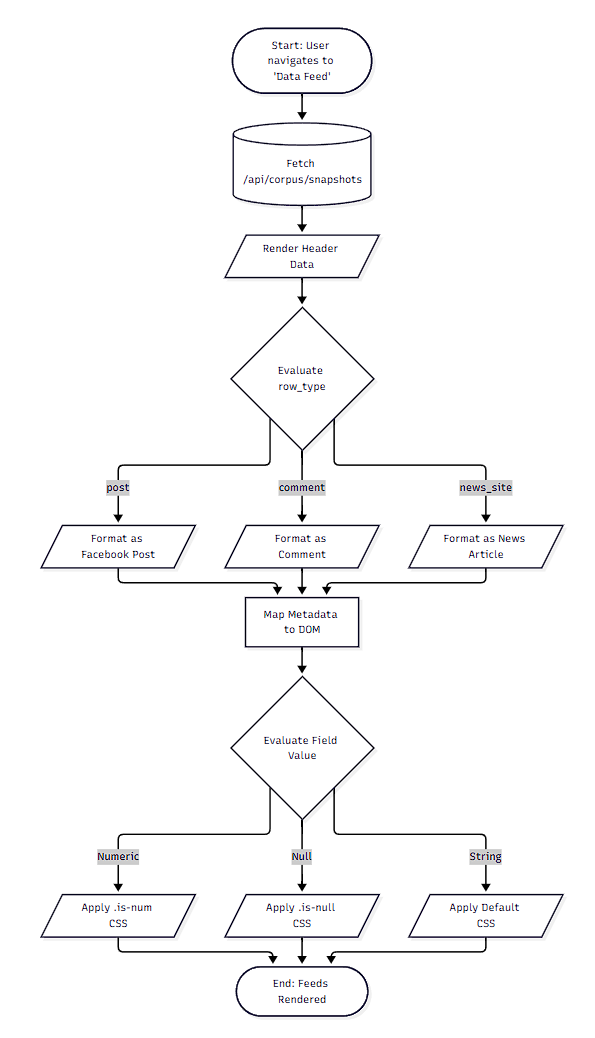
\includegraphics[width=0.5\textwidth]{figures/image1.png}
	\caption{Data Feed Integration}
	\label{fig:data_feed_integration}
\end{figure}

This figure \ref{fig:data_feed_integration} details the extraction and dynamic DOM mapping of the 10,194-report corpus, displaying how conditional styling is applied based on raw metadata attributes.

\begin{figure}[htbp]
	\centering
	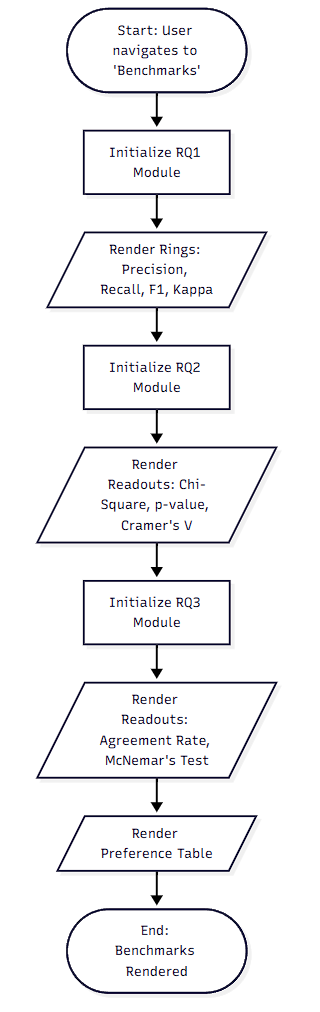
\includegraphics[width=0.4\textwidth]{figures/image4.png}
	\caption{Algorithm Benchmarks}
	\label{fig:algorithm-benchmarks}
\end{figure}
This figure \ref{fig:algorithm-benchmarks} demonstrates the sequential rendering process of the statistical evaluation modules, summarizing the data visualization for Research Questions 1, 2, and 3.

\begin{figure}[htbp]
	\centering
	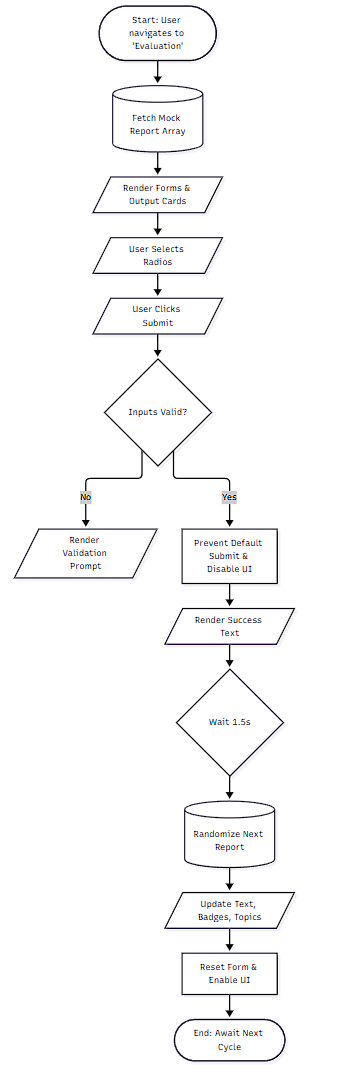
\includegraphics[width=0.4\textwidth]{figures/image3.png}
	\caption{Blind stakeholder evaluation}
	\label{fig:blind-stakeholder-evaluation}
\end{figure}
This figure \ref{fig:blind-stakeholder-evaluation} demonstrates the sequential rendering process of the statistical evaluation modules, summarizing the data visualization for Research Questions 1, 2, and 3.

\subsection*{Research Question 1: Joint Matrix Latent Topic Structure and
	Sentiment Classification Relationship Analysis}

Regarding Research Question 1, an assessment is conducted to determine whether a
relationship exists between the respective joint matrices of \sysA{} and \sysB{}
and how strong the association is between their joint matrices' topics and sentiment classifications. This must be done to analytically
justify that the two systems have the ability to capture the topics and
sentiments of Facebook posts during natural disasters, and their quantifiable
measures of performance in doing so.

\paragraph{Bivariate Analysis.} As a statistical method, bivariate analysis
serves as an analytical tool that determines the empirical relationship between
two variables, their interaction with one another, trends, and possible causal
relationships. It aims at examining the relationship between two variables to
gain insight into whether such a relationship exists, how strong it is, and
whether it is positive or negative. By examining this, it allows a
quantifiable understanding of two variables \parencite{bennd}. Since our joint
matrix is composed of topics and sentiment classifications, this can be
interpreted as two variables that the study seeks to analytically determine
whether their joint matrix is significantly associated.

Within this investigation, the system-generated topics and sentiment
classifications from the joint matrices of both systems will serve as the two
variables evaluated for bivariate analysis. Prior to performing further
bivariate analysis using the Chi-Square Statistic and Fisher's Exact Test, the output
must be in the form of a cross-tabulation to create a structured framework of
computation in matrix format. The joint matrix itself is a form of bivariate
analysis, as it is a cross-tabulation or contingency table that allows us to
see the frequency distribution of both variables in the same format and gives
insight into their associations \parencite{bennd}.

\paragraph{Chi-Square Statistic Test.} The chi-square test is used to determine
whether there is a significant difference between observed frequencies and
expected frequencies and, in contingency tables, the relationship between
categorical variables. It can be used to determine whether a significant
relationship exists between two or more variables. This association can be
negative, positive, or an absence of association. To test whether an association
exists, we set the null hypothesis that no association exists and the
alternative hypothesis that an association exists. To decide whether to reject
or fail to reject the null hypothesis, we first compute the chi-square statistic
($\chi^2$) and obtain the critical value to determine whether we conclude that
no association exists or that an association exists.The formula to attain $\chi^2$ is
\begin{equation}
	\chi^2 = \sum_{i=1}^{R} \sum_{j=1}^{C}
	\frac{\left(O_{ij} - E_{ij}\right)^2}{E_{ij}}
	\label{eq:chisq}
\end{equation}
where $R$ is the number of rows of the joint matrix (the topics), $C$ is
the number of columns of the joint matrix (the sentiment classifications),
$O_{ij}$ are the observed frequencies in the joint matrix---the actual raw count
of Facebook posts that either of the two systems assigns to latent topic $i$ and
sentiment classification $j$---and $E_{ij}$ are the expected frequencies, or
the calculated marginal totals of the matrix if the null hypothesis is true. To
attain $E_{ij}$, the formula is
\begin{equation}
	E_{ij} = \frac{R_i \, C_j}{n}
	\label{eq:expected}
\end{equation}

For determining thresholds, we need to test $\chi^2$ against the chi-square
distribution table; to attain that, we first need the degrees of freedom $df$:
\begin{equation}
	df = (R - 1)(C - 1)
	\label{eq:df}
\end{equation}
After this, a Python function is used to determine the critical value; it takes
the contingency table as its input, and if the associated $p$-value is less
than the chosen significance level, the null hypothesis is rejected and the
joint matrix is deemed to have a significant association \parencite{singh2020}.

\paragraph{Fisher's Exact Test.} 
The Chi-Square tests needs to be applied with caution for contingency tables that might have cells that has low frequencies as the statistical model itself has a continous distribution while the underlying data might be discontinuous. It is stated that for Chi-Square test to be applied several assumptions are to be followed:
\begin{enumerate}
	\item all cells of the contingency table must be $>1$
	\item atleast 80\% of all cells should be $>5$
\end{enumerate}

This limitations by the Chi-Square was addressed by the Fisher's Exact Test. It utilizes the hyper-geometric distribution to calculate the probabilities. When utilizing this model it is conservative in achieving a fixed significance level due to the hyper-geometric distribution being highly discrete in small samples. The model can be extended beyond the 2x2 contingency table by utilizing the Freeman-Halton extension\parencite{mays2026fisher}.

\begin{equation}
	P = \frac{\prod_{i=1}^{R} R_i! \prod_{j=1}^{C} C_j!}{n! \prod_{i=1}^{R} \prod_{j=1}^{C} x_{ij}!}	
	\label{eq:fisher}
\end{equation}

Conditioned on fixed row totals $R_i$ and columns total $C_j$. It also has $N$ as grand total of the table and $n_{ij}$ for the count in cell $(i,j)$ \parencite{metricgate2026freeman}.

\subsubsection{Acceptability Thresholds}

The resulting performance measures will be examined to confirm whether a relationship exists on the topics and sentiment classifications within the joint matrix of both \sysA{} and \sysB{}.

A $p < 0.05$ conventional rejects the null hypothesis for both Chi-Square and Fisher's Exact Test implying there is a relationship between variables and population \parencite{mays2026fisher}. This performance measures will be applied
independently to both \sysA{} and \sysB{} before a relative comparative
analysis that evaluates their relative performance with one another.


\subsection*{Research Question 2: Blind Stakeholder Evaluation}

Research Question 2 evaluates the stakeholder assessment regarding the outputs
generated by \sysA{} and \sysB. From the common evaluation corpus, a randomly
selected sample will be examined through a blind evaluation procedure in which
the order of the systems' outcomes will be randomized. A simple majority rule
will determine the aggregation rule for each document, because the identity of
the system making each output will not be revealed to the evaluators. When this
evaluation takes place, agreement, differences in ratings, and paired
assessment outcomes will be considered. Each evaluator is expected to evaluate
50--100 randomly sampled documents drawn from the outputs of \sysA{} and
\sysB.

\paragraph{McNemar's Test.} For stakeholder evaluation, paired binary results
will be examined using McNemar's Test, which is suitable for systematic
comparisons when identical assessors evaluate two systems in two categories.
The test statistic incorporates continuity correction:
\begin{equation}
	\chi^2_{\text{McNemar}} = \frac{\left(\lvert b - c \rvert - 1\right)^2}{b + c}
	\label{eq:mcnemar}
\end{equation}
In the calculation, $b$ indicates cases where \sysA{} succeeds while \sysB{}
fails, and $c$ indicates cases where \sysB{} succeeds while \sysA{} fails. This
comparison aims to reveal operational differences, with the $p$-value being
analyzed to assess the statistical significance of the differences between the
outcomes of the two systems.

\subsubsection*{Acceptability Thresholds}

The resulting performance measures will be examined to confirm whether a
statistically significant difference exists between the paired outcomes of
\sysA{} and \sysB{} when assessing overall performance.

An Agreement Rate of at least 70\% is deemed acceptable as high agreement in
inter-rater reliability \parencite{stemler2004}. Meanwhile, a McNemar's Test at the
0.05 significance level will be the minimum acceptability threshold
\parencite{mcp2025}; that is, a system has alignment of the sentiment classification and topic identification of stakeholders around natural disasters in Bulacan and the CAMANAVA area in the same sampled facebook posts or comments in the processed corpus, as it
indicates a detection of possible differences between the system and the assessments
stakeholders around the same sampled items. These performance measures will be applied to both \sysA{} and \sysB{}.

\section*{Respondents and Expert Evaluators of the Study}

The development and comparative evaluation of the SAKLOLO. natural language
processing pipeline requires highly specialized domain expertise rather than
general population sampling. Consequently, the study utilizes a purposive
sampling design to form a Blind Evaluation Stakeholder Panel.

\subsection*{Exclusion of Population-Based Sample Size Formulas}

When determining the number of evaluators for natural language processing (NLP)
architectures, traditional probabilistic calculations (such as Cochran's or
Slovin's formulas) are mathematically and methodologically incompatible with
the research design. These formulas are designed for epidemiological or
sociological surveys where the goal is to achieve a representative demographic
cross-section of a generalized population. They assume that every member of the
population has an equal probability and capacity to provide valid data.

The evaluation of the proposed framework, however, is not a demographic survey
but rather an experimental computational benchmark. The study requires human
evaluators to audit the classification outputs of a hybrid pipeline
(LDA + XLM-RoBERTa) and an open-weight transformer $Qwen3-1.7B-Instruct-Q4\_K\_M$.

Evaluating contextual embeddings, coherence, and algorithmic classification
disparities requires calibrated judgment from domain specialists. Using a
purposively selected expert panel provides the controlled conditions necessary
to execute specific non-parametric statistical validations (such as McNemar's
test and rank correlation coefficients) to detect genuine differences in model
configurations without introducing data dilution.

\subsection*{Blind Evaluation Stakeholder Panel (System Evaluation)}

To execute the blind comparative evaluation between the lightweight hybrid model
(\sysA: LDA + \xlmr) and the state-of-the-art open-weight
(\sysB: $Qwen3-1.7B-Instruct-Q4\_K\_M$), a total panel of 10 to 20 evaluators will be recruited. This panel is
divided equally into two specialized cohorts.

\begin{table}[htbp]
	\centering
	\caption{Cohort A and Cohort B Descriptions}
	\label{tab:cohorts}
	\begin{tabularx}{\textwidth}{XX}
		\toprule
		\textbf{Cohort A: DRRM Operational Officers ($n = 5$--$10$)} &
		\textbf{Cohort B: Academic and Technical Experts ($n = 5$--$10$)} \\
		\midrule
		\textit{Source.} Active personnel, incident commanders, and communication
		dispatchers from the Provincial and Municipal Disaster Risk Reduction and
		Management Offices (DRRMOs) of the Bulacan and CAMANAVA corridors. &
		\textit{Source.} Faculty members and researchers specializing in Applied
		Mathematics, Computer Science, and Data Analytics, specifically targeting
		the Mathematics Department of the College of Science and the allied faculty
		of the CICT at Bulacan State University. \\
		\addlinespace
		\textit{Operational Role.} These practitioners evaluate the practical
		applicability, operational fidelity, and functional alignment derived from
		the models without knowing which system generated the output. They provide
		judgment on whether the extracted sentiment and disaster urgency accurately
		reflect actual field conditions. &
		\textit{Operational Role.} These experts assess the mathematical validity
		and thematic coherence of the extracted topic probabilities and contextual
		embeddings, ensuring the algorithms operate within accepted standards of
		information theory and machine learning rigor. \\
		\bottomrule
	\end{tabularx}
\end{table}

\begin{table}[htbp]
	\centering
	\caption{Summary of Study Participants}
	\label{tab:participants}
	\begin{tabularx}{\textwidth}{XXXXX}
		\toprule
		\textbf{Participant Group} & \textbf{Target Size ($n$)} &
		\textbf{Sampling Method} & \textbf{Target Affiliation} &
		\textbf{Research Function} \\
		\midrule
		DRRM Practitioner Panel & 5--10 & Purposive &
		Bulacan and CAMANAVA DRRM Offices &
		Blind evaluation of system outputs; assesses operational applicability and relevance. \\
		\addlinespace
		Academic Technical Panel & 5--10 & Purposive &
		Mathematics and Computer Science Faculty (College of Science / CICT) &
		Technical validation of thematic coherence, joint embeddings, and
		comparative algorithmic quality. \\
		\addlinespace
		\textbf{Total Panel} & \textbf{10--20} & \textbf{Purposive} & --- & --- \\
		\bottomrule
	\end{tabularx}
\end{table}

In software engineering and machine learning benchmark literature, evaluating
models against human baselines relies on expert panel auditing rather than
large-scale probability sampling. A focused panel of calibrated domain
specialists provides the necessary statistical power to execute paired
nonparametric tests---specifically McNemar's test for classification disparity,
preference ratio calculations, and Cohen's Kappa for inter-system
consensus---while eliminating evaluation fatigue and ensuring reliable
judgments.

\section*{Research Instrument}

The research instrument of the study is a structured blind evaluation form. It
is meant to assess the agreement of stakeholder assessments with the outputs of
\sysA{} and \sysB. The instrument is designed to allow both systems to be
evaluated independently using the same sampled disaster-related textual
documents while concealing the identity of the producing system.

The stakeholder will assess whether the two presented sentiment classifications
agree with their own assessment of the document using a multiple choice for human sentiment of the sampled content to test alignment of the respective system's alignment with human experts on that subject. The same procedure is to be applied to the topic output of the two systems in a yes or no format. The evaluation form records the stakeholder's assessment for
each system output and the corresponding identifiers. These responses are to be
converted into agreement observations for statistical analysis. The instrument
is to be administered with the same instructions, response categories, and
evaluation conditions for all participating stakeholders to maintain consistency
across observations.

\section*{Ethical Considerations}

This study observes ethical considerations for the safety of participants and
maintains the integrity of this paper throughout the development of
\emph{SAKLOLO: A Hybrid Semantic-Probabilistic Framework for Analysing Social
	Media Emergency Feeds in Bulacan and CAMANAVA}. The researchers will follow
ethical guidelines such as collecting data from identified sources, obtaining
consent, ensuring the confidentiality of participants and voluntary
participation, using social media responsibly, and maintaining integrity in
presenting the research results for transparency. Appropriate procedures are
established to maintain confidentiality and to protect the privacy of all
participants in this study. The study adheres to the following ethical
principles:

\begin{description}[style=nextline,leftmargin=0pt]
	\item[Data Privacy and Confidentiality.] Republic Act No. 10173, or the Data
	Privacy Act of 2012, establishes the rights of individuals needed to protect
	their personal information, and the organization is responsible for the
	personal information of participants \parencite{ra10173}. The needed
	disaster-related report data will be processed only if needed, solely for
	this study. The study will exclude unnecessary personal information. The
	study will focus on collecting disaster-related information from identified
	sources such as social media and DRRM reports in Bulacan and CAMANAVA. This
	data will be filtered to remove irrelevant data and personal information for
	the privacy and accuracy of the study. All collected data are for academic
	research and model validation purposes only \parencite{npc2016}.
	
	\item[Voluntary Participation and Informed Consent.] Participants will be
	informed about the purpose and procedure of this study prior to their
	involvement. Participants in this study are voluntary; they have the right to
	decline to participate in this study without penalty. To ensure accuracy and
	prevent biases during evaluation, a protocol will be established wherein
	evaluators will be anonymized without being informed whether the predictions
	were from the LLM baseline model or the hybrid pipeline system
	\parencite{belmont1979}.
	
	\item[Confidentiality of Participants.] The identity of participants and
	personal information of stakeholders will be kept confidential in this study.
	The evaluation process will use a blind evaluation procedure so that the
	system does not reveal the identity of evaluators. Possible data that can
	identify participants will be excluded from the results to prevent biases and
	to protect the participants. In accordance with the Data Privacy Act of 2012
	\parencite{ra10173, npc2016}, the identity of participants shall be protected
	against alteration and unauthorized access.
	
	\item[Responsible Use of Social Media Data.] Only data relevant to the study
	will be collected, such as disaster-related data from publicly accessible
	social media of DRRM offices. The usernames of commenters from social media
	and other personal identifiers will be excluded from the data collection
	process. The researchers ensure that social media will be used responsibly
	and solely for academic purposes, not to harm anyone. Moreover, all collected
	data from social media will be anonymized and processed in accordance with
	ethical research standards \parencite{npc2016}.
	
	\item[Research Integrity.] The researchers of this study uphold transparency,
	honesty, and objectivity throughout the development of the study. All data
	related to this study, such as evaluations and results, will be properly
	collected and studied accurately without falsification and fabrication. This
	study will be developed ethically and honestly, and results will be presented
	with integrity whether the outcome is expected or not \parencite{belmont1979}.
	This study ensures reliability, credibility, and transparency. Moreover,
	citations to all sources such as DRRM reports, social media posts, and other
	materials will be properly acknowledged within the paper.
\end{description}
	
	\printbibliography
\end{document}